% =====================================================================
%  Neural Demodulation of Hardware-Captured PSK and Star-QAM Waveforms
%  With a Bounded Input Context
%  (retitled 2026-10-30 in response to the two technical reviews; was
%  "Under a Provable Memorisation Bound")
%
%  Target: IEEE Access
%
%  TEMPLATE
%  This is the IEEE Access build of the manuscript. It uses the official
%  ieeeaccess.cls from ACCESS_latex_template_20260513. The class,
%  spotcolor.sty, IEEEtran.cls, IEEEtran.bst, the Formata/Times/Giovanni
%  fonts and the IEEE Access logos all sit in this directory, so the paper
%  compiles with a plain pdflatex run and needs nothing installed. The
%  untouched template, including IEEE's own sample document access.tex and
%  its access.pdf, is kept in ./access-template/.
%
%  The IEEEtran build in ../paper-ieeetran/ has NOT been updated with the
%  2026-10-30 revision; its body no longer matches this file.
%
%  ieeeaccess.cls loads IEEEtran and hyperref itself, so neither is loaded
%  here. The front matter below uses the Access commands: \history, \doi,
%  \address, \tfootnote, \corresp, and an abstract that must precede
%  \maketitle.
%
%  OUTSTANDING BEFORE SUBMISSION
%   1. refs.bib was checked against Crossref, arXiv and DataCite on
%      2026-10-31 (see its header). Table I codings for studies before 2025
%      come from the hand-filled worksheet and were not re-read.
%   2. Fig. 1: relabel the five boards individually as B1-B5.
%   3. \history and \doi carry IEEE's placeholder values; IEEE fills them in.
%   4. Numbers added in the 2026-10-30 revision come from src/:
%      context_bound.py (Table VI, ISI, filter support, context and
%      position-only controls), classical_lopo.py (Table VII classical),
%      run_revision.py (extra seeds, partitions, latent head),
%      run_experiments.py (corrected shuffled-label control), and
%      revision_tables.py (Tables VII, VIII, X). Figs. 4-6 are drawn by
%      src/figures.py and copied into figures/ here. The positive control
%      (Section VI, tab:positive, added 2026-10-31) comes from
%      window_control.py -> results/window_control.csv; print its table with
%      "window_control.py --summary". The trace-readability control
%      (Section VI-C) comes from isi_readability.py ->
%      results/isi_readability.csv.
%   5. AI-use and WorldCUR disclosures (draft notes in the Acknowledgment).
% =====================================================================

\documentclass{ieeeaccess}

\usepackage[T1]{fontenc}   % accented names in the bibliography need T1
\usepackage{cite}
\usepackage{amsmath,amssymb,amsfonts}
\usepackage{graphicx}
\usepackage{textcomp}
\usepackage{booktabs}
\usepackage{multirow}
\usepackage{url}

% Bold math set up for the Access fonts; carried over from the template.
\usepackage{bm}
\makeatletter
\AtBeginDocument{\DeclareMathVersion{bold}
\SetSymbolFont{operators}{bold}{T1}{times}{b}{n}
\SetSymbolFont{NewLetters}{bold}{T1}{times}{b}{it}
\SetMathAlphabet{\mathrm}{bold}{T1}{times}{b}{n}
\SetMathAlphabet{\mathit}{bold}{T1}{times}{b}{it}
\SetMathAlphabet{\mathbf}{bold}{T1}{times}{b}{n}
\SetMathAlphabet{\mathtt}{bold}{OT1}{pcr}{b}{n}
\SetSymbolFont{symbols}{bold}{OMS}{cmsy}{b}{n}
\renewcommand\boldmath{\@nomath\boldmath\mathversion{bold}}}
\makeatother

\graphicspath{{figures/}}
\newcommand{\SER}{\mathrm{SER}}

% ---------------------------------------------------------------------
% Draft notes. Unwritten sections must be VISIBLE in the PDF: a LaTeX
% comment renders as nothing, so a section awaiting content looks broken
% rather than pending. Set \draftfalse before submission and every note
% disappears; nothing else changes.
% ---------------------------------------------------------------------
\newif\ifdraft
\drafttrue          % <<< SET TO \draftfalse BEFORE SUBMISSION
\newcommand{\todonote}[2]{%
  \ifdraft
    \par\medskip\noindent
    \fbox{\parbox{0.94\columnwidth}{\footnotesize
      \textbf{[TO WRITE --- #1]}\\[2pt]#2}}%
    \par\medskip
  \fi}

\begin{document}

\history{Date of publication xxxx 00, 0000, date of current version xxxx 00, 0000.}
\doi{10.1109/ACCESS.2024.0429000}

\title{Neural Demodulation of Hardware-Captured PSK and Star-QAM Waveforms
With a Bounded Input Context}

\author{\uppercase{Mohammad Khalid Hasan Nabil}\authorrefmark{1},
\uppercase{Ivan Grgi\'{c}}\authorrefmark{2},
AND \uppercase{Md. Maynul Islam}\authorrefmark{1}}

\address[1]{Department of Information and Communication Technology, Bangladesh
University of Professionals, Dhaka 1216, Bangladesh (e-mail:
nabil23549009015@student.bup.edu.bd; maynul.mist@gmail.com)}

\address[2]{Mechanical Engineering Faculty in Slavonski Brod, University of
Slavonski Brod, 35000 Slavonski Brod, Croatia (e-mail: igrgic@unisb.hr)}

\tfootnote{Dataset, trained models, and analysis code are available at
\url{https://github.com/not-your-pancake/Ai-demod} and archived via Zenodo at
\url{https://doi.org/10.5281/zenodo.23509606}.}

\markboth
{M. K. H. Nabil \headeretal: Neural Demodulation With a Bounded Input Context}
{M. K. H. Nabil \headeretal: Neural Demodulation With a Bounded Input Context}

\corresp{Corresponding author: Mohammad Khalid Hasan Nabil (e-mail:
nabil23549009015@student.bup.edu.bd).}

% =====================================================================
\begin{abstract}
% Learned receivers are commonly evaluated on data whose transmitted sequence is
% short and periodic, which allows a sufficiently expressive model to reproduce
% the sequence from context rather than demodulate the waveform. We present a
% hardware dataset and a receiver design in which this failure mode is excluded by
% construction. Waveforms were captured from five physically distinct
% communication trainer boards across BPSK, QPSK and a four-phase two-amplitude
% star 8-QAM constellation, yielding 43 oscilloscope records and 154{,}628
% labelled symbols. Ground-truth labels are obtained by coherent averaging of the
% transmitted waveform rather than from the transmitter's configuration, and are
% verified independently: all sixteen BPSK captures reproduce the board's 63-bit
% maximal-length sequence exactly, and a single memoryless mapping explains three
% distinct QPSK data words simultaneously ($p < 5\times10^{-5}$). Because the
% transmitted sequence has linear order six, any six consecutive bits determine
% the seventh; we therefore restrict the receiver's input to at most five bits,
% making prediction-from-context impossible rather than merely improbable. A
% 21{,}000-parameter convolutional receiver operating on the raw passband waveform
% attains symbol error rates statistically indistinguishable from a blind
% matched-filter receiver across all three modulations, while receiving neither
% the carrier frequency, the pulse shape, nor the constellation geometry. Holding
% out an entire data word costs $0.005$ in symbol error rate relative to a random
% split, and on that split both a shuffled-label control and a signal-free
% positional control remain at chance. We additionally report two negative
% results: a constellation-geometry loss term does not improve error rate, and a
% widely suggested carrier-sensitivity comparison does not survive measurement.

Learned receivers are often evaluated on data whose transmitted sequence is short and periodic, which lets an expressive model predict a symbol from its neighbours
instead of demodulating it. We bound this failure mode by construction: 
each input window holds fewer neighbouring symbols than are needed to determine its label, verified 
for every transmitted word by enumerating the measured labels. We test 
it on 154,628 hardware-captured symbols from five trainer boards across 
BPSK, QPSK and star 8-QAM. Labels are measured from the waveform, and 
Gaussian noise is added in software. A 21,000-parameter convolutional receiver on symbol-synchronous 
passband windows, given neither the carrier frequency nor the constellation, comes close to a classical reference receiver that 
is given both: at the lowest signal-to-noise ratio its 8-QAM symbol error rate is 8.6\% higher. The bound does not exclude 
partial predictability of the context, nor a trace of neighbouring symbols about 20 dB below the symbol's energy. 
Empirically, the receiver does no better on a random split, where such cues would help, than on held-out words 
with comparable training data. A positive control confirms the test: given a window past the bound, the same 
network labels symbols it cannot see on a random split, yet fails on held-out words even without noise. 
Holding out one of the five boards costs more. Two negative results are reported: a constellation-aware 
loss term does not improve accuracy and its latent output collapses, and a commonly proposed carrier-sensitivity disadvantage of classical receivers does not hold up under measurement.

\end{abstract}

\begin{IEEEkeywords}
Neural receiver, demodulation, deep learning, physical layer, hardware dataset,
maximal-length sequence, memorisation, symbol error rate, quadrature amplitude
modulation.
\end{IEEEkeywords}

\titlepgskip=-21pt

\maketitle

% =====================================================================
\section{Introduction}
\IEEEPARstart{L}{earning}-based receivers recover digital modulation from
sampled waveforms without an explicitly specified signal
model~\cite{oshea2017intro,dorner2018ota,ye2018power}. A recurring difficulty in
evaluating such systems is that the transmitted data is frequently a short
pseudorandom sequence repeated many times. When that is so, a model with
sufficient temporal context can predict the next symbol from preceding symbols
alone, without extracting any information from the waveform. The reported error
rate then measures sequence memorisation rather than demodulation, and held-out
evaluation does not detect this if the same short sequence appears in both
partitions.

This paper bounds the failure mode by construction and then tests what the
bound leaves open. For every transmitted word we compute, from the measured
symbol-label sequence, the shortest neighbouring context that determines a
symbol exactly. The receiver's input window is cut so that the neighbouring
symbols it contains always fall short of that length. No window therefore
determines its own label by lookup, whatever the network's capacity or
training. The bound is a property of the data presented to the network
rather than of its architecture, and it can be checked by enumeration. It is
also narrower than an impossibility result. A short context can still be
partly predictive, and the transmitter's pulse response leaves a weak trace
of neighbouring symbols inside the window. We measure both, and we use held-out
words and a corrected shuffled-label control to test whether the receiver
exploits them. A positive control then removes the bound. Given a longer
window, the same network memorises the transmitted words; a random split
rewards this, and held-out words expose it. The evaluation can therefore detect
the failure it is designed to exclude.

The contributions are as follows.

\begin{enumerate}
\item A hardware dataset of 43 dual-channel oscilloscope captures from five
physically distinct trainer boards, spanning BPSK, QPSK and a two-ring star
8-QAM constellation, with a per-record verification protocol and full
provenance (Section~\ref{sec:dataset}).
\item A ground-truth procedure based on coherent averaging of the transmitted
waveform. The recovered BPSK labels reproduce the transmitted bit sequence and
the QPSK labels fit a single symbol mapping. The 8-QAM labels are verified as
constellation-point classes only (Section~\ref{sec:groundtruth}).
\item A bounded-context input design. For every transmitted word, the
neighbouring symbols inside a window are too few to determine the window's
label, which we verify by enumerating the measured label sequences. We also
measure what the bound does not exclude: partial predictability of the
context, and inter-symbol interference from the transmitter. A positive
control, the same network with the bound removed, shows that held-out words
detect the memorisation that a random split rewards
(Sections~\ref{sec:bound}, \ref{sec:generalisation}, \ref{sec:controls}
and~\ref{sec:positive}).
\end{enumerate}

Three side results are reported briefly. A constellation-geometry loss term
does not improve error rate, and its latent output collapses to a single point
(Section~\ref{sec:geometry}). A classical receiver's dependence on carrier
knowledge is not a practical disadvantage at any observation length tested
(Section~\ref{sec:limitations}). The boards' own demodulators show a lock
threshold that reproduces across all five units, and an unlocked demodulator
can still give a self-consistent output (Section~\ref{sec:hardware}).

We make no claim of improved error-rate performance, and the network is a
small, conventional one-dimensional CNN. The contributions are the dataset and
the evaluation design. The learned receiver comes
close to a classical reference receiver but does not match it at the lowest
signal-to-noise ratios (Section~\ref{sec:ser}). The contribution is that it gets
this close without being given the carrier frequency, the constellation
geometry or the decision boundaries. It still uses symbol-synchronous windows
and record-level gain control, and its input cannot determine a label from
context alone.

% =====================================================================
\section{Related Work}
\label{sec:related}

\subsection{Learned physical-layer processing}
Learned physical-layer processing has been demonstrated for end-to-end
autoencoder transceivers~\cite{oshea2017intro}, for systems trained over the
air~\cite{dorner2018ota}, and for joint channel estimation and
detection~\cite{ye2018power}. Modulation classification from sampled in-phase
and quadrature data has received particular attention, together with the
synthetic datasets used to benchmark it~\cite{satyanarayan2023RML}. Broad
reviews of the area are given in~\cite{hoydis2021nativeAirInterface,
akroutMLPtoGPT, wangDlphysicalLayer}, and of distribution shift specifically
in~\cite{akrout2023domaingeneralization}.

The useful axis for comparison is what each system is \emph{given}.
Table~\ref{tab:related_a} records, for twenty-one recent learned receivers and
demodulators, whether the carrier frequency, the symbol timing, the pulse shape
and the constellation are supplied rather than recovered, together with the
domain of the input and the origin of the evaluation data. The RML22 dataset
paper~\cite{satyanarayan2023RML} and the 6G vision
article~\cite{hoydis2021nativeAirInterface} are cited above but not tabulated,
because neither evaluates a receiver of its own.

The distribution is uneven. Nine operate on baseband in-phase and quadrature
samples and seven on frequency-domain subcarriers; four take symbols already at
the output of a matched filter, and one operates on passband samples.
Fifteen are given the carrier frequency and fourteen the symbol timing.
Eighteen are given the constellation, and seventeen fix a known pulse-shape
family without presenting it to the network. Nineteen are evaluated on
simulated waveforms only. Of the two exceptions, Hanna \textit{et al.} use
hardware captures for validation~\cite{Hanna2022SignalProcessing}, and
Cammerer \textit{et al.} also train their system over the air on software-defined
radios~\cite{cammerer2020trainableCS}.

\begin{table*}[!t]
\caption{What recent learned receivers and demodulators are given.
\emph{family} denotes a fixed known pulse-shape family that is not itself
presented to the network; \emph{blind} denotes symbol timing recovered by the
system; \emph{partial} denotes a residual offset estimated from the signal;
\emph{n.s.} denotes a property the paper does not state, which is not the same
as a property it does not use. \emph{Domains}: passband, baseband in-phase and
quadrature, post-matched-filter symbols, frequency domain. \emph{Data}: simulated,
hardware used for validation only, hardware also used for over-the-air training
(\emph{hw-train}), hardware as the primary source. Surveys, datasets and vision
articles without an evaluated receiver are cited in the text and not tabulated.}
\label{tab:related_a}
\centering
\begin{tabular}{lcccccc}
\toprule
System & Carrier & Timing & Pulse & Const. & Domain & Data \\
\midrule
Zhu \textit{et al.}~\cite{Zhu2022WaveformLevelIntelligence} & yes & blind & family & no & baseband & sim. \\
Zhu \textit{et al.}~\cite{Zhu2022EndtoEnd} & yes & blind & family & yes & baseband & sim. \\
Hanna \textit{et al.}~\cite{Hanna2022SignalProcessing} & partial & blind & family & yes & baseband & hw-valid. \\
Xiao \textit{et al.}~\cite{Xiao2023_UnifiedDeep} & no & blind & family & no & baseband & sim. \\
Zhu \textit{et al.}~\cite{Zhu2023DLWave} & yes & blind & family & yes & baseband & sim. \\
Chia \textit{et al.}~\cite{Chia2022RN} & yes & yes & family & yes & baseband & sim. \\
Tonix-Gleason \textit{et al.}~\cite{Tonix2025NNAided} & yes & yes & family & yes & freq. & sim. \\
Liu \textit{et al.}~\cite{liu2026Universal} & yes & yes & family & yes & freq. & sim. \\
Zhang \textit{et al.}~\cite{Zhang2018Enhanced} & no & blind & family & yes & passband & sim. \\
Dakic \textit{et al.}~\cite{dakic2021LoRa} & no & blind & family & yes & baseband & sim. \\
Zheng \textit{et al.}~\cite{Zheng2022DemodNet} & no & yes & yes & yes & symbols & sim. \\
Allwin \textit{et al.}~\cite{alwin2024LLRSymNet} & yes & yes & yes & yes & symbols & sim. \\
Gansekoele \textit{et al.}~\cite{ganse2024MLApprochDemapping} & yes & yes & yes & yes & symbols & sim. \\
Polvani \textit{et al.}~\cite{polvani2021MIMO} & yes & yes & yes & yes & symbols & sim. \\
Wang \textit{et al.}~\cite{wang2024optimalSequence} & yes & yes & family & yes & baseband & sim. \\
Chen \textit{et al.}~\cite{chen2024robustSymboldetection} & yes & yes & family & yes & freq. & sim. \\
Gorday \textit{et al.}~\cite{gorday2020complexNN} & no & yes & family & yes & baseband & sim. \\
Fischer \textit{et al.}~\cite{fischer2022OFDM} & yes & yes & family & yes & freq. & sim. \\
Honkala \textit{et al.}~\cite{honkala2021deeprxfullyconvolutionaldeep} & yes & yes & family & yes & freq. & sim. \\
Korpi \textit{et al.}~\cite{korpi2021UplinkCNN} & yes & yes & family & yes & freq. & sim. \\
Cammerer \textit{et al.}~\cite{cammerer2020trainableCS} & yes & yes & family & no & freq. & hw-train \\
\addlinespace
This work & no & yes & family & no & passband & hw-primary \\
\bottomrule
\end{tabular}
\end{table*}

A minority withhold more. Zhang \textit{et al.} demodulate BPSK with a
sliding-window one-dimensional convolutional network on raw passband samples,
detecting phase-shift locations without explicit carrier synchronisation or
symbol-period grouping~\cite{Zhang2018Enhanced}; that system is the closest to
ours in input domain, and differs in being evaluated on simulated waveforms and
in being given the constellation. Xiao \textit{et al.} take raw baseband samples
and compensate time and frequency offsets blindly while jointly predicting the
modulation type and the symbol index~\cite{Xiao2023_UnifiedDeep}. Dakic
\textit{et al.} predict LoRa symbols directly from baseband samples and report
robustness to emulated carrier and time offsets without explicit synchronisation
modules~\cite{dakic2021LoRa}. Zhu \textit{et al.} recover bit sequences from
oversampled baseband sequences while handling symbol timing offsets blindly
through a shifted binary cross-entropy loss~\cite{Zhu2022EndtoEnd}. Hanna
\textit{et al.} estimate carrier offset, timing and symbol rate blind and then
decode with a minimum-distance receiver against the classified modulation's
constellation~\cite{Hanna2022SignalProcessing}, and are one of the two entries
whose evaluation involves hardware.

The larger group operates in the frequency domain with synchronisation already
established. DeepRx performs channel estimation, equalisation and soft demapping
jointly and emits bit log-likelihood ratios for
5G~\cite{honkala2021deeprxfullyconvolutionaldeep}, and its MIMO extension adds
either a combining-based or a fully learned transformation
layer~\cite{korpi2021UplinkCNN}. Cammerer \textit{et al.} train a bit-wise
autoencoder that learns geometric constellation shaping and bit labelling
jointly with iterative demapping and decoding~\cite{cammerer2020trainableCS},
making it one of the three tabulated systems not given a constellation. A
further group learns the demapping alone, from symbols already at the
matched-filter output~\cite{Zheng2022DemodNet, alwin2024LLRSymNet,
ganse2024MLApprochDemapping, polvani2021MIMO}.

These systems are evaluated on held-out partitions. Eleven of the twenty-one
report a random held-out split; the remaining ten do not state one. None
reports a partition grouped by recording or by device, and none constrains the
receiver's input context relative to the context complexity of the transmitted
sequence, which is the property Section~\ref{sec:bound} imposes by
construction.

\subsection{Evaluation validity and memorisation}
This paper's premise is that held-out evaluation is insufficient when the
transmitted sequence is short and periodic. Related concerns are long-standing
in machine learning generally---train/test contamination, and models that
exploit dataset artefacts rather than the intended signal---but the specific
failure considered here is narrower: the test sequence itself is predictable
from its own past, so a model with sufficient context can reach a low error rate
without demodulating.

Work in radio-frequency sensing has begun to quantify the effect. In a recent
preprint, Shulman reports that segment-level cross-validation causes severe
data leakage and optimism in drone identification benchmarks, and that
regrouping the evaluation by recording brings the inflated accuracies down to
chance~\cite{shulman2026rfdronebenchmarksoverstate}; among the studies
surveyed here it is the only one that reports a recording-grouped split. The
same failure is documented outside wireless: Brookshire \textit{et al.} show
that dividing recordings into segments without grouping by subject produces
severe leakage and heavily inflated performance in translational
electroencephalography studies~\cite{brook2024dataLeakage}.

The underlying concern is long-standing in machine learning generally. Carlini
\textit{et al.} give a quantitative framework for testing whether a sequence
model has unintentionally memorised rare training
sequences~\cite{nicolas2019secretSharer}, and Arpit \textit{et al.} show that
gradient-based optimisation learns simple patterns before it memorises
noise~\cite{arpit2017memorizationinDL}. These results establish that the
partition matters, and that memorisation is measurable after training. None of
them limits, before training begins, what context a receiver can draw on.
Among the learned-receiver studies reviewed here, none constrains receiver
context below the context complexity of the test sequence. That gap is part of
the motivation for Section~\ref{sec:bound}.

\subsection{Hardware-captured RF datasets}
Public RF datasets are commonly synthesised, or captured from a small number of
transmitters with ground truth asserted from the transmitter's configuration
rather than measured from the emitted waveform. The distinction matters here:
Section~\ref{sec:dataset} shows a case in which the configured data word is
\emph{not} a reliable statement of the transmitted symbol sequence, and
Section~\ref{sec:groundtruth} obtains labels by measurement instead.

Table~\ref{tab:related_c} lists twelve public radio-frequency datasets against
three axes: the number of physical devices, the granularity of the labels, and
whether the data are captured from hardware or simulated. Nine are captured
primarily from hardware, one uses hardware for validation only, and two are
simulated.

\begin{table}[!t]
\caption{Public radio-frequency datasets. \emph{n.s.} denotes a quantity the
dataset does not state; \emph{n/a} denotes a category that does not apply. The
device counts are as reported. Ours is smaller than every stated count except
the three of~\cite{saria2019droneRF}.}
\label{tab:related_c}
\centering
\begin{tabular}{lrll}
\toprule
Dataset & Devices & Label & Source \\
\midrule
Hanna \textit{et al.}~\cite{hanna2022WiSig} & 174 & device & hw-primary \\
Vrieze \textit{et al.}~\cite{vrieze2018earnestRF} & n.s. & mod.-class & hw-primary \\
Al-Shawabka \textit{et al.}~\cite{amani2020fingerprint} & n.s. & device & hw-valid. \\
Elmaghbub \textit{et al.}~\cite{bub2021usecase} & 25 & device & hw-primary \\
Zahid \textit{et al.}~\cite{zahid2025comrad} & 27 & device & hw-primary \\
Morin \textit{et al.}~\cite{Morin2019Transmitter} & 20 & device & hw-primary \\
Utrilla~\cite{Utrilla2020MIGOU-MOD} & n.s. & mod.-class & hw-primary \\
Allahham \textit{et al.}~\cite{saria2019droneRF} & 3 & mod.-class & hw-primary \\
Kashani \textit{et al.}~\cite{kashani2024BLE} & 13 & device & hw-primary \\
Jagannath \textit{et al.}~\cite{jagannat2024commercialDevice} & 10 & device & hw-primary \\
Jaensch \textit{et al.}~\cite{jaensch2024radiomapestimation} & n/a & radio map & sim. \\
Yapar \textit{et al.}~\cite{yapar2024datasetpathlosstoaradio} & n/a & radio map & sim. \\
\addlinespace
This work & 5 & symbol & hw-primary \\
\bottomrule
\end{tabular}
\end{table}

The axis that matters here is label granularity. Seven of the twelve label at
device level and three at modulation-class level. The remaining two are
radio-map datasets whose targets are path loss and time of arrival rather than
properties of a received signal. None labels individual symbols. Hanna \textit{et al.} release the
largest, ten million packets from 174 transmitters recorded across 41 receivers
over a month~\cite{hanna2022WiSig}; Elmaghbub \textit{et al.} capture 25 LoRa
transceivers across indoor, outdoor and wired
testbeds~\cite{bub2021usecase}; Zahid \textit{et al.} capture 27
radios~\cite{zahid2025comrad}; Morin \textit{et al.}
twenty~\cite{Morin2019Transmitter}; Kashani \textit{et al.}
thirteen~\cite{kashani2024BLE}; and Jagannath \textit{et al.} ten commercial
chipsets~\cite{jagannat2024commercialDevice}. Our five units are fewer than any
of these, and far fewer than the 174 of~\cite{hanna2022WiSig}.

The distinction we draw is therefore not scale but what a label denotes. The
datasets above answer which device transmitted a signal, or which modulation it
carries. A symbol-level label answers which constellation point was transmitted
at a given instant, which is what a demodulator must predict, and which
Section~\ref{sec:groundtruth} obtains by measurement from the waveform rather
than by assertion from the transmitter's configuration.

\subsection{Classical receiver theory}
Classical treatments of the receiver functions replaced by learned
systems---carrier recovery, timing recovery, matched filtering and
detection---are given in~\cite{proakis2007digital} and~\cite{mengali1997sync}.
The timing-error detector referenced in Section~\ref{sec:limitations} is due
to~\cite{gardner1986ted}. Properties of maximal-length sequences, including the
linear recursion used in Section~\ref{sec:bound}, are standard and are set
out in~\cite{golomb1982shift}.

% =====================================================================
\section{Experimental Setup and Dataset}
\label{sec:dataset}

\subsection{Apparatus}
Signals were captured from MCM31/EV communication trainer boards using a
two-channel digital oscilloscope, shown in Fig.~\ref{fig:setup}. Channel~1
observes TP-20, the modulated output, and channel~2 observes TP-9, the board's
own recovered data. The two are acquired simultaneously so that network input
and hardware baseline originate from a single record. Acquisition is externally
triggered from the board's symbol clock at TP-1.

\begin{figure*}[!t]
\centering
% Printed at 0.80\textwidth rather than full width. The source photograph is
% 1280 px across, which is 179 dpi at full text width -- below the 220 dpi IEEE
% asks for on photographs -- and 223 dpi at this width. Scaling an image down
% raises its effective resolution; scaling it up would not add information.
% If a higher-resolution original of the photograph becomes available, restore
% width=\textwidth.
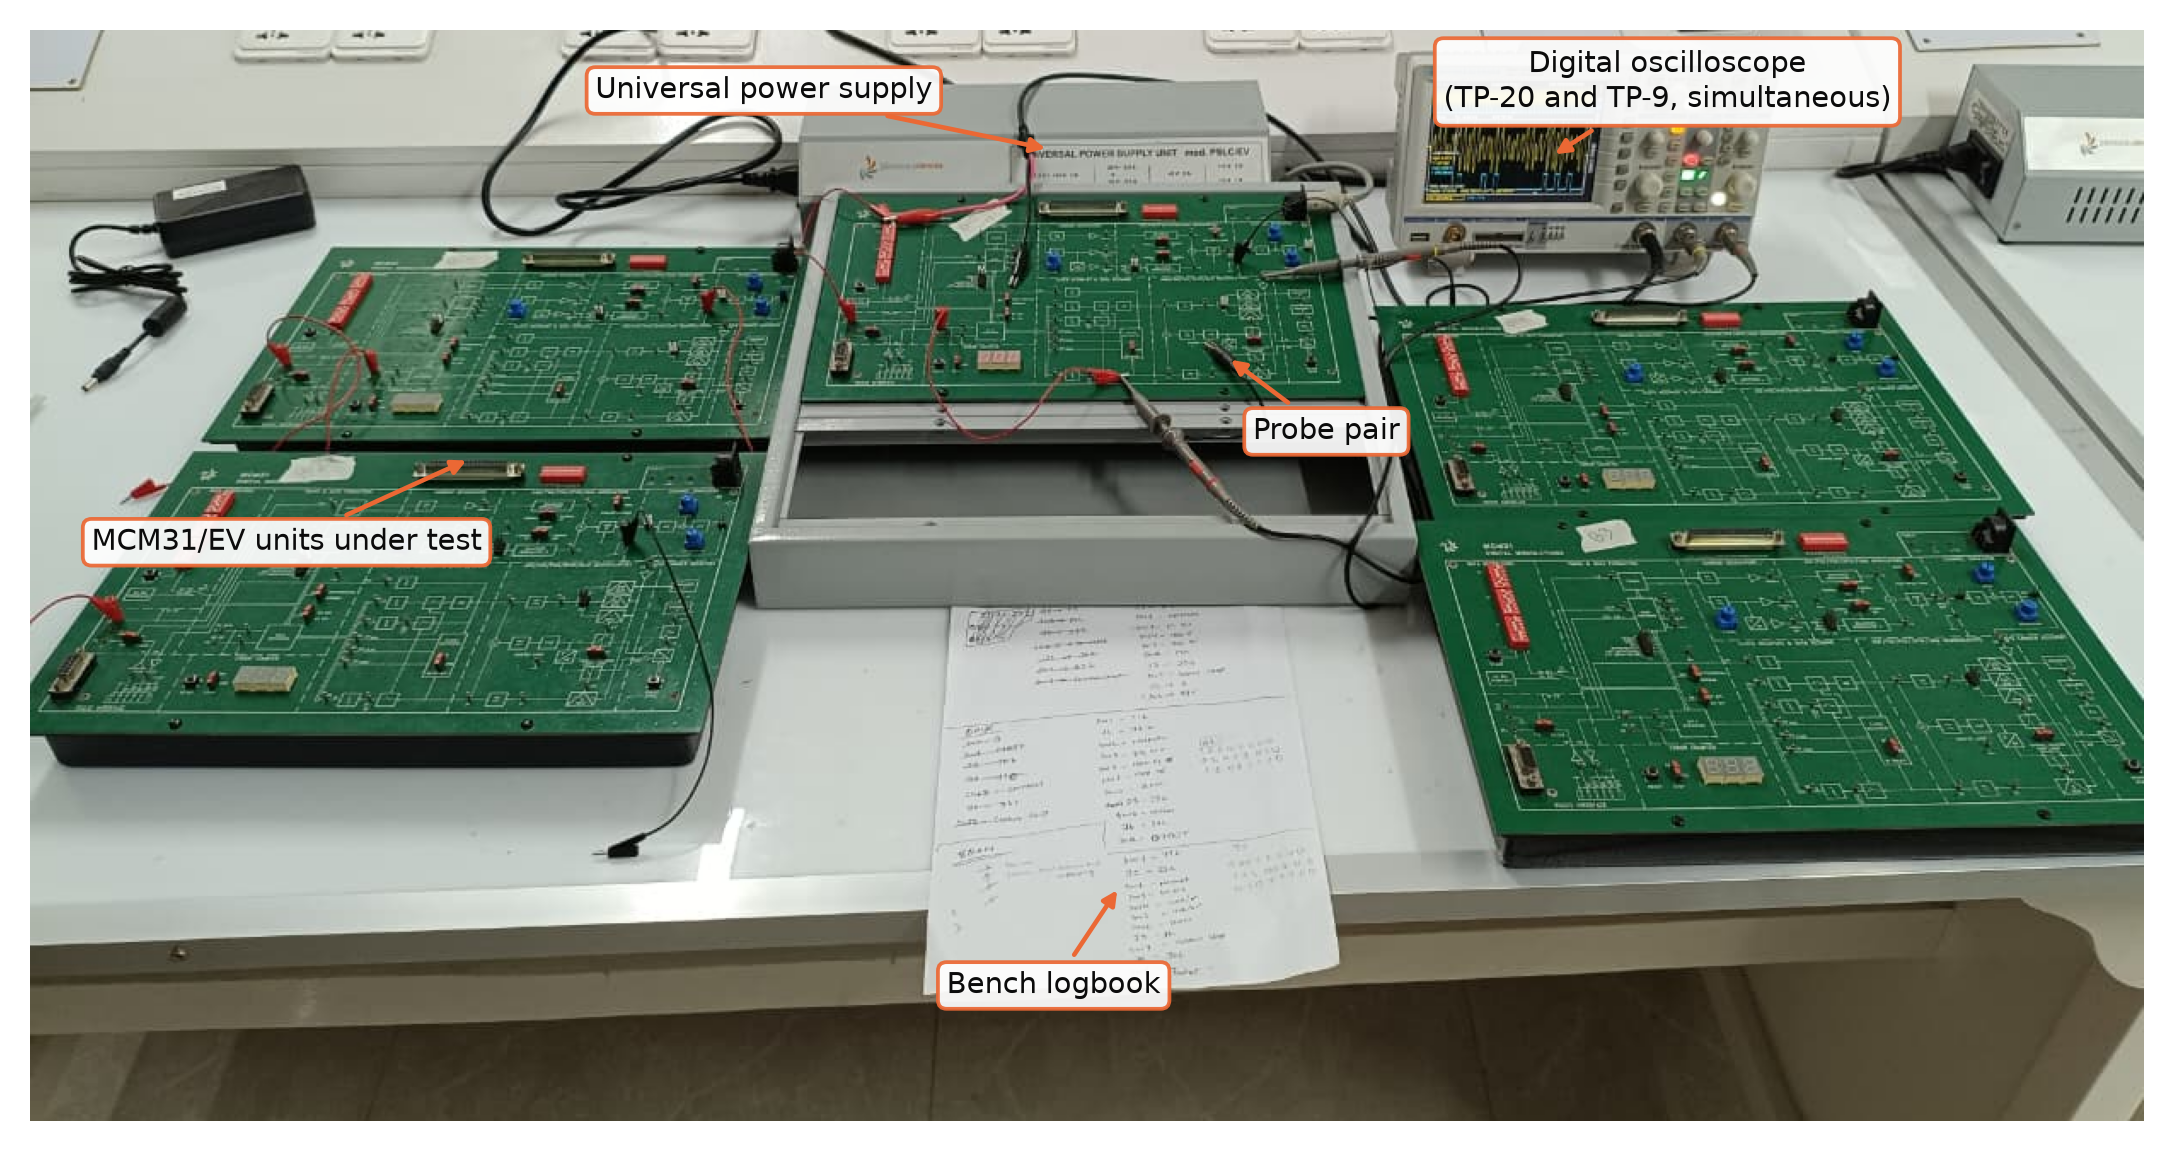
\includegraphics[width=0.80\textwidth]{fig0_setup.png}
\caption{Measurement bench. The five MCM31/EV trainer units, labelled Board-1 to
Board-5, correspond to boards B1--B5 in Table~\ref{tab:perfold} and
Fig.~\ref{fig:lock}. One unit is under test at a time, powered from a shared
supply, with the oscilloscope probing TP-20 and TP-9 simultaneously and
triggered externally from TP-1.}
\label{fig:setup}
\end{figure*}
\todonote{Fig.~1 board labels}{Both reviews note that Board-1 to Board-5 are not
legible on the photograph. Add visible B1--B5 annotations to fig0\_setup.png.}

Acquisition parameters were fixed for every record and are given in
Table~\ref{tab:acq}. The time base was chosen so that each record contains at
least 57 repetitions of the longest data word, which is what makes the coherent
averaging of Section~\ref{sec:groundtruth} effective. A shorter time base was
evaluated and rejected: it yields too few repetitions for a stable
signal-to-noise estimate.

\begin{table}[!t]
\caption{Acquisition and signal parameters. All values were measured from the
captured records rather than taken from the equipment specification.}
\label{tab:acq}
\centering
\small
\begin{tabular}{ll}
\toprule
Parameter & Value \\
\midrule
Sample rate & $87{,}260$~Sa/s \\
Samples per record & $523{,}600$ \\
Record duration & $6.0004$~s \\
Channel 1 & TP-20, modulated output \\
Channel 2 & TP-9, recovered data \\
Trigger & external, from TP-1 \\
\midrule
Carrier & $1199.91$~Hz \\
Symbol rate & $599.955$~baud \\
Carrier cycles per symbol & $2$ (exact) \\
Samples per symbol & $145.44$ \\
\midrule
BPSK data source & on-board 63-bit m-sequence \\
QPSK, 8-QAM data source & 24-bit configurable words \\
\bottomrule
\end{tabular}
\end{table}

The carrier is coherent with the symbol clock at exactly two cycles per symbol.
This is the property that permits coherent averaging: the passband waveform
repeats exactly at the word period, so averaging over repetitions suppresses
noise without distorting the signal.

\subsection{Units under test}
Ten units were sourced. Five were functional; five were excluded following
individual inspection, in each case because the on-board data generator had
failed, either in the sequence-load latch or in the pseudorandom generator
itself. On such a unit the modulator receives no data and TP-20 carries an
unmodulated carrier: the coherent template contains all of its energy in the
carrier bin and none in the sidebands, and no usable waveform exists to capture.
All results below therefore rest on five boards, and leave-one-board-out is a
five-fold evaluation.

\subsection{Per-record verification}
Every record was subjected to the battery of checks in Table~\ref{tab:checks}
before admission to the corpus. The battery is not decorative: it rejected
records during the campaign and each rejection corresponded to a real
configuration fault.

\begin{table}[!t]
\caption{Per-record verification battery. Every record in the corpus passes
every check except where noted in Section~\ref{sec:dataset}-D.}
\label{tab:checks}
\centering
\small
\begin{tabular}{clc}
\toprule
Check No. & Check & Pass condition \\
\midrule
1  & Channel count            & 2 channels present \\
2  & Sample count             & $520{,}000$--$526{,}000$ \\
3  & Duration                 & $5.99$--$6.01$~s \\
4  & Sample rate              & $87{,}000$--$87{,}500$~Sa/s \\
5  & Quantisation levels      & $\geq 90$ distinct \\
6  & Carrier (4th power)      & $1199.5$--$1200.5$~Hz \\
7  & Word-period repetition   & $r \geq 0.95$ \\
8  & Coherent-template SNR    & $\geq 15$~dB \\
9a & Same word, two records   & similarity $\geq 0.99$ \\
9b & Constellation fingerprint & matches the expected word \\
9c & Different words          & similarity $< 0.99$ \\
10 & TP-9 agreement           & logged, not gating \\
\bottomrule
\end{tabular}
\end{table}

Elaborating check No.(9a--9c) from Table~\ref{tab:checks}, we see that check No.~(9a) compares two records of the same
configured word and detects a failure to reload the transmitter between
captures. Check No.~(9b) compares the multiset of per-constellation-point occupancy
counts against the value predicted by the configured word; it is invariant to
constellation rotation and to the mapping between transmitter configuration and
transmitted symbol, and therefore identifies the loaded word without assuming
that mapping. Check No.~(9c) is the converse and is required for held-out words, each
of which is captured only once: two \emph{different} configured words must not
produce the same waveform. Neither (9a) nor (9b) detects a stale word in that case,
because words designed to cover the full constellation share a fingerprint by
construction.

Check No.~(9c) must be evaluated on the \emph{signed} similarity. Two words that are
bitwise complements produce waveforms that are exact negations of one another,
and an unsigned similarity reports these as identical when they are merely
antipodal.

\subsection{Corpus}
The corpus comprises 43 records: fifteen from board~B1 (seven main-campaign
records and eight additional data words held out for evaluation) and seven from
each of B2--B5. Segmentation at the symbol rate yields $154{,}628$ labelled
symbols, distributed as in Table~\ref{tab:dataset}. Coherent-template SNR across
the accepted corpus is $22.7$--$43.2$~dB, median $30.2$~dB.

The design is not fully crossed. The primary words PRBS63, Q1 and T1 are
recorded on all five boards: PRBS63 three times per board and Q1 and T1 twice.
The additional words S1, Q2, Q3 and T2--T6 are recorded once each, on B1 only.
Pattern identity and board identity are therefore confounded for those words.
A leave-one-pattern-out fold that withholds one of them tests a new word on
B1, not a new word on unseen hardware.

\begin{table}[!t]
\caption{Dataset composition. \emph{Words} counts distinct configured bit
patterns; \emph{independent} accounts for the antipodal equivalence described in the text.
}
\label{tab:dataset}
\centering
\begin{tabular}{lrrrr}
\toprule
Modulation & Records & Symbols & Words & Independent \\
\midrule
BPSK  & 16 & 57{,}536 & 2 & 2 \\
QPSK  & 12 & 43{,}152 & 3 & 3 \\
8-QAM & 15 & 53{,}940 & 6 & 5 \\
\midrule
Total & 43 & 154{,}628 & & \\
\bottomrule
\end{tabular}
\end{table}

The distinction between \emph{words} and \emph{independent patterns} for 8-QAM is
material. Two of the six words are bitwise complements of one another, and on
this hardware complementary tribits map to antipodal constellation points: their
coherent templates correlate at $-0.998$. After per-record amplitude
normalisation the two carry identical information, and we therefore treat them
as a single pattern throughout. Counting them separately would bias the
leave-one-pattern-out result optimistically.

Four of the six 8-QAM words deliver six of the eight constellation points rather
than the eight their bit patterns specify. The discriminator is a property
computable from the bit pattern alone: a word is \emph{framing robust} if all
eight tribits survive every cyclic bit rotation. The two robust words deliver
eight points; the four fragile words deliver six. This is consistent with the
transmitter grouping bits into tribits from a fixed offset that does not
coincide with the configuration order. It does not affect the labels, which are
measured from the waveform, but it does mean the configured word is not a
reliable statement of the transmitted symbol sequence which is precisely why
the ground-truth procedure of Section~\ref{sec:groundtruth} does not use it.

\subsection{Measured constellations}
Fig.~\ref{fig:constellation} shows every symbol of every record, pooled across
the five boards. The 8-QAM constellation is a four-phase, two-amplitude star of
measured radius ratio $1.89$ (range $1.867$--$1.914$ over fifteen records). It is
not a rectangular 16-QAM grid, and a loss function assuming rectangular geometry
is inconsistent with this hardware.

\begin{figure*}[!t]
\centering
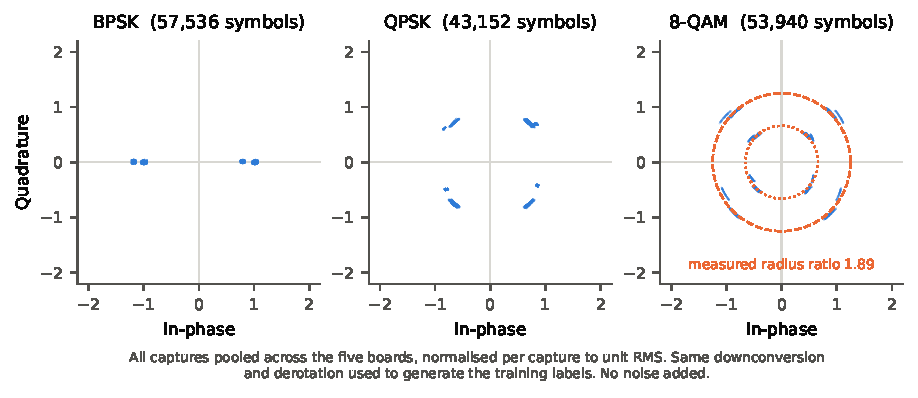
\includegraphics[width=\textwidth]{fig_constellation.pdf}
\caption{Measured constellations: individual symbols, not the coherently
averaged template. Each symbol is downconverted and integrated over its own
symbol interval. Each record is derotated by its own whole-record $m$th-power
estimate \eqref{eq:derotate} and normalised to unit RMS. All records are
pooled across the five boards, and 6{,}000 symbols per panel are drawn at
random. The spread therefore shows per-symbol capture variability, including
device-to-device differences. The 8-QAM panel shows the two rings at the
measured radius ratio of $1.89$. No noise has been added.}
\label{fig:constellation}
\end{figure*}

% =====================================================================
\section{Ground Truth}
\label{sec:groundtruth}

Labels are derived from the transmitted waveform, not from the transmitter's
configuration. Fig.~\ref{fig:pipeline} shows the two processing paths and their
separation.

\begin{figure*}[!t]
\centering
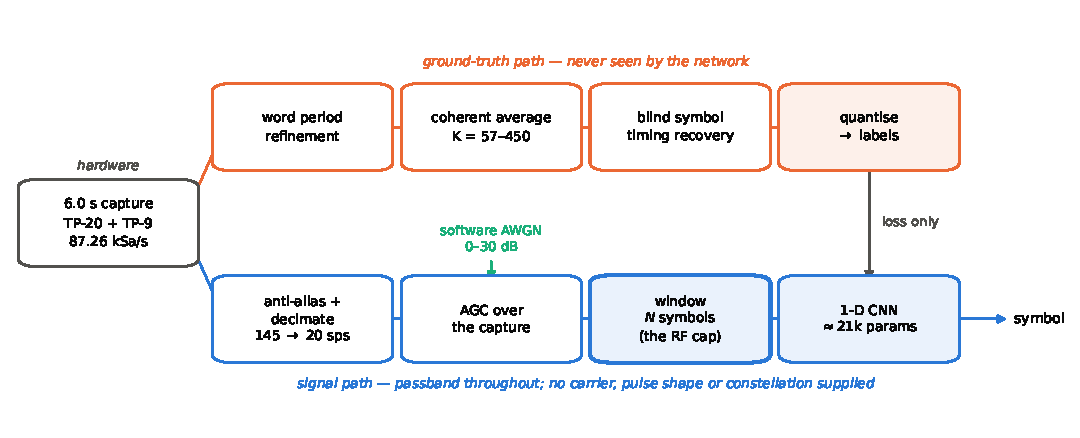
\includegraphics[width=\textwidth]{fig_pipeline.pdf}
\caption{Processing chain. The upper path produces ground-truth labels by
coherent averaging; the lower path produces the network's input. The paths share
the raw capture, and also the word period and the symbol timing $\tau^{\star}$
estimated from the coherent template. The network's windows are cut on the
symbol grid that $\tau^{\star}$ defines, a dependency not drawn in the diagram.
The label path reads the same filtered, resampled waveform from which the
windows are cut (Section~\ref{sec:groundtruth}-B). At training and test time,
software noise is added to each window first, and the window is then divided
by its record's noise-free RMS (Section~\ref{sec:conditioning}). Labels reach
the network only through the loss.}
\label{fig:pipeline}
\end{figure*}

\subsection{Coherent averaging}
Let $x[n]$ be the captured passband waveform and $P$ the word period in samples,
which is not in general an integer. The record is folded into $K$ segments
resampled onto a common grid of $M = \lfloor P \rceil$ points,

\begin{equation}
\begin{split}
x_k[m;P] = x\!\left(kP + m\tfrac{P}{M}\right)\!, \quad &k = 0, \dots, K-1, \\
&m = 0, \dots, M-1,
\end{split}
\label{eq:fold}
\end{equation}

and the template is their mean,
\begin{equation}
t[m;P] = \frac{1}{K}\sum_{k=0}^{K-1} x_k[m;P].
\label{eq:template}
\end{equation}
The period is refined by maximising the energy of the coherent average,
\begin{equation}
P^{\star} = \arg\max_{P} \ \operatorname{var}_m\big(t[m; P]\big),
\label{eq:period}
\end{equation}
searched over $\pm 6$ samples in steps of $0.02$ samples with $M$ held fixed so
that candidates are scored on a common grid. Writing
$\sigma_r^2 = \operatorname{var}(x_k[m] - t[m])$ for the residual variance, the
template signal-to-noise ratio is reported as
\begin{equation}
\mathrm{SNR}_t = 10\log_{10}
\frac{\operatorname{var}(t) - \sigma_r^2/K}{\sigma_r^2},
\label{eq:tsnr}
\end{equation}
in which the second numerator term removes the averaging bias, so the quantity
reported is the single-repetition signal-to-noise ratio rather than the
flattered post-averaging one.

\subsection{Symbol extraction}
To prevent the final symbol from falling on the wrap boundary, the coherent template is first extended circularly prior to filtering. The subsequent downconversion is achieved without requiring an external carrier estimate; because the transmitted word contains exactly $2N_s$ carrier cycles for $N_s$ symbols, the downconverted sequence is computed as:
\begin{equation}
b[n] = t_{\mathrm{ext}}[n] \, e^{-j 2\pi (2N_s) n / M},
\label{eq:downconv}
\end{equation}
where $b[n]$ represents the downconverted discrete-time signal sequence, $t_{ext}[n]$ is the circularly extended coherent template waveform, $n$ is the discrete-time sample index,$N_s$ denotes the total number of transmitted symbols within the data word, and $M$ is the number of grid points per word established in Section IV-A. This formulation remains exact regardless of the underlying sample rate. 

Following downconversion, the sequence $b[n]$ is passed through a one-symbol boxcar, the matched filter for a rectangular pulse. Symbols are then sampled at instants $(i+\tau)T_s$, where $T_s$ is the symbol period. The fractional timing offset $\tau \in [0, 1)$ is recovered without data aid, by maximising the mean symbol magnitude on a $1/256$-symbol grid refined to $1/4096$:
\begin{equation}
\tau^{\star} = \arg\max_{\tau} \ \frac{1}{N_s}\sum_{i} \big| s_i(\tau) \big| .
\label{eq:timing}
\end{equation}
where $s_i(\tau)$ denotes the complex filter output for the $i$-th symbol evaluated at the candidate timing offset $\tau$, and $i$ represents the discrete symbol index. Symbol-timing recovery is a prerequisite rather than a refinement. Extracting symbols without Equation (6) places decision instants part-way through transitions and collapses individual constellation radii—in our data, two of the eight 8-QAM radii fell to 0.20 against a nominal 1.31. This artefact is visually indistinguishable from a template wrap-boundary error and must be excluded before that diagnosis is reached. 

Once timing is established, the residual constellation rotation is removed by an $m$th-power estimate:
\begin{equation}
\rho = \frac{1}{m}\arg\!\left(
  \mathbb{E}\!\left[s^m\right] e^{-j m \phi_{\mathrm{ref}}}\right),
\qquad s' = s\,e^{-j\rho},
\label{eq:derotate}
\end{equation}
where $\rho$ is the estimated residual rotation angle, $m$ is the modulation-dependent exponent ($m = 2$ for BPSK and $m = 4$ otherwise), and $\phi_{ref}$ is the target reference phase for the constellation. The variable $s$ represents the optimally sampled complex symbol (corresponding to $s_i(\tau^*)$), $s'$ is the resulting derotated symbol, and $\mathbb{E}[\cdot]$ denotes the sample mean taken over all $\approx 3600$ symbols of the capture record.   The rotation $\phi_{ref}$ must be applied inside the argument as written: for a reference phase of $45^\circ$, the fourth-power sum lies near $180^\circ$, which sits on the branch cut of the argument function. Subtracting the phase afterwards would erroneously place records whose phase is physically identical $90^\circ$ apart. Furthermore, the expectation is calculated over the entire record rather than a single word, because a single word covering the constellation unevenly introduces enough bias to select an incorrect quadrant. Either of these errors would relabel every symbol of the affected record while leaving all per-record diagnostics deceptively intact.

The template supplies only the word period and $\tau^{\star}$. The labels are computed from the whole record, on the filtered, resampled waveform of Section~\ref{sec:conditioning}, whose symbol grid is set by $\tau^{\star}$. Each symbol is downconverted at exactly two carrier cycles per symbol and integrated over its own interval. All symbols of the record are derotated by \eqref{eq:derotate} and averaged over the $K$ repetitions of the word. The averaged word is then quantised. BPSK classes are the sign of the real part. QPSK classes are the phase quadrant. 8-QAM classes are the phase quadrant plus one bit for whether the radius exceeds the word's median radius. The word labels are tiled over the record. This whole procedure is offline: it uses the complete record, and nothing like it is available to the network at inference.

Because $\phi_{\mathrm{ref}}$ is fixed, the labelling convention is common to all records. A class index refers to the same constellation point in every record. The evidence is that all $148$ pairs of records carrying the same word, including pairs from different boards and attenuations, have label sequences identical up to a cyclic shift (Section~\ref{sec:controls}).

\subsection{Verification of the labels}
Two checks test the recovered labels against what was transmitted. They do not
give the same confirmation for every modulation.

\begin{enumerate}
\item BPSK has sixteen records. The fifteen PRBS63 records reproduce the board's
63-bit maximal-length sequence at $100\%$, against a chance level of $66.6\%$
(95th percentile $69.8\%$). The chance level is computed over 63 cyclic shifts
and both polarities. The one record of the 24-bit word S1 reproduces S1 at
$100\%$ under the same search. The carrier is recovered by fourth-power
estimation at $1199.915$--$1199.918$~Hz across all five boards.
\item A single memoryless bijection from constellation point to dibit fits all
three QPSK data words simultaneously at $100\%$---36 symbols explained by one
four-point mapping. Across $20{,}000$ label permutations preserving the
per-symbol occupancy counts, a perfect fit never occurred, giving
$p < 5\times10^{-5}$.
\end{enumerate}

The second check also resolves, for BPSK and QPSK, the mapping between
transmitter configuration and transmitted symbol. For 8-QAM it cannot: a word
covering all eight points exactly once admits a perfect bijection for any
rotation, so the test is vacuous for a single word and remains unresolved.

The verified claims therefore differ by modulation. For BPSK, the label
sequences are confirmed as the transmitted bit sequences. For QPSK, they are
consistent with a single memoryless dibit mapping. For 8-QAM, the labels are
measured constellation-point classes. They are confirmed only by the
occupancy fingerprint of check~9b and by the cross-record consistency above.
Which tribit each class carries is not established. Every 8-QAM result in this
paper concerns recovery of constellation-point classes, not of transmitted bits.
The context analysis of Section~\ref{sec:bound} uses the measured class
sequences, which is the target the network is trained on. It therefore does
not depend on the unresolved tribit mapping or on the framing offset.

The classical reference receiver of Section~\ref{sec:ser} is not independent of
this procedure. It uses the same downconversion, integration, derotation and
decision regions, but on single noisy symbols rather than on a word averaged
over $57$--$450$ repetitions. Its agreement with the labels at high
signal-to-noise ratio is therefore expected by construction. It is a reference
for the error rate the labels permit, not an independent check of the labels.

% =====================================================================
\section{Receiver}

This section defines what the receiver sees and how it is evaluated: the
bounded input window (Section~\ref{sec:bound}), the signal conditioning and
noise model (Section~\ref{sec:conditioning}), the network and its training
(Section~\ref{sec:arch}), and the evaluation splits.

\subsection{The bounded input context}
\label{sec:bound}
\emph{Window geometry.} The network receives a window of $N$ consecutive
symbols and labels the symbol at a fixed position within it:
$[t{-}2,\,t{-}1,\,t,\,t{+}1,\,t{+}2]$ for BPSK, $[t{-}1,\,t]$ for QPSK and
$[t]$ for 8-QAM, where $t$ is the target. The \emph{neighbouring} content of a
window is therefore four symbols for BPSK (two on each side), one preceding
symbol for QPSK, and none for 8-QAM. The target's own waveform is the signal to
be demodulated and is not counted as context.

\emph{Context complexity.} Let $y_0,\dots,y_{L-1}$ be the cyclic sequence of
measured labels of one word, with indices taken modulo $L$. Its one-sided
context complexity $\kappa^{-}$ is the smallest $k$ for which $y_i$ is a
function of $(y_{i-k},\dots,y_{i-1})$ at every position $i$. The two-sided
complexity $\kappa^{\pm}$ is the smallest $k$ for which $y_i$ is a function of
the $\lfloor k/2\rfloor$ preceding and $k-\lfloor k/2\rfloor$ following labels.
If a window's neighbouring content is shorter than this, some context in the
word occurs with two different labels. No lookup, however learned, can then
recover every label of the word from its neighbours. The quantities are
computed on the measured label sequences, which are the targets the network is
trained on, not on the configured bit strings. They are invariant to cyclic
shift and to any fixed relabelling of the classes, so the unresolved 8-QAM
tribit mapping does not affect them.

For PRBS63 the property also follows from the sequence's linear recursion. The
bit string as listed for the board is the complement of the maximal-length
sequence that satisfies
\begin{equation}
s[i+6] = s[i] \oplus s[i+5],
\label{eq:lfsr}
\end{equation}
where $s[i]$ is the $i$-th bit of that sequence and $\oplus$ is modulo-2
addition~\cite{golomb1982shift}. Complementing every bit leaves every context
property unchanged. Six consecutive bits determine the next one exactly; five
do not. Thirty-one of the thirty-two five-bit patterns occur twice per period,
once followed by each bit. The all-zero pattern occurs once and is followed by
a one. Even a one-sided five-bit context therefore predicts the next bit at no
more than $32$ of $63$ positions. The configured 24-bit words obey no such
recursion: their minimum one-sided bit contexts are six to nine bits, and their
symbol-level complexities are found by enumeration (Table~\ref{tab:context}).

\begin{table}[!t]
\caption{Context complexity of every measured word, in symbols. \emph{Window}
is the neighbouring context each window contains. \emph{Lookup} is the
accuracy of the best lookup from that context to the target label within the
word, as if the neighbours were known without error. \emph{Chance} is
$1/(\text{number of classes})$.}
\label{tab:context}
\centering
\begin{tabular}{llrrcrr}
\toprule
Mod. & Word & $\kappa^{-}$ & $\kappa^{\pm}$ & Window & Lookup & Chance \\
\midrule
BPSK  & PRBS63 & 6 & 10 & 2+2 & 0.508 & 0.500 \\
BPSK  & S1     & 7 &  7 & 2+2 & 0.625 & 0.500 \\
QPSK  & Q1     & 3 &  4 & 1+0 & 0.417 & 0.250 \\
QPSK  & Q2     & 3 &  3 & 1+0 & 0.583 & 0.250 \\
QPSK  & Q3     & 2 &  3 & 1+0 & 0.333 & 0.250 \\
8-QAM & T1+T2  & 1 &  1 & 0   & 0.125 & 0.125 \\
8-QAM & T3--T6 & 2 &  2 & 0   & 0.250 & 0.125 \\
\bottomrule
\end{tabular}
\end{table}

Every window falls short of its word's complexity, and the margins explain the
caps. A third QPSK symbol would supply two preceding symbols, enough to
determine every label of Q3. A second 8-QAM symbol would supply one, enough for
T1 and T2, in which each of the eight points occurs exactly once per word. The
BPSK cap of five symbols is conservative.

\emph{What the bound does not exclude.} It excludes one thing exactly:
deterministic lookup of a label from the neighbouring symbols in its window. It
does not make the context uninformative. The \emph{Lookup} column exceeds
chance for S1 and for all three QPSK words, so a context cue could still act as
a prior at low signal-to-noise ratio. Section~\ref{sec:controls} measures that
cue on the actual splits.

The bound also counts symbols, not signal dependence. Two mechanisms carry
neighbouring-symbol information into a window. The first is the digital front
end. The zero-phase anti-alias filter of Section~\ref{sec:conditioning} has a
two-sided support of $257$ raw samples, $\pm 0.88$ symbol. A window sample can
therefore depend on raw samples outside its own symbol interval. The filter's
response is concentrated, though: only $-50$~dB of its energy lies beyond
$\pm 0.5$ symbol. The second mechanism is the transmitter's own pulse response,
which no front end removes. We measure it on the word-averaged, noise-free
waveform. For each symbol, we take the deviation of its 20 samples from the
mean of all symbols of the same class; only its neighbours can cause that
deviation. Relative to the symbol's own RMS, the deviation is $-18.5$ to
$-18.9$~dB for BPSK, $-21.0$ to $-25.2$~dB for QPSK, and $-24.2$ to $-27.9$~dB
for the 8-QAM words in which a point repeats. In units of half the minimum distance between class means, it
is $0.12$, $0.08$--$0.16$ and $0.17$--$0.21$. A one-symbol 8-QAM window
therefore carries a weak trace of its neighbours. The bound applies to the
symbols explicitly present in the digital window, not to every transmitted bit
that can influence its samples.

That trace has a consequence that the comparison of splits is designed to
test. For T1 one preceding symbol determines the label, so on a split whose
test records carry a training word, a receiver able to read the previous symbol
through the trace could look its label up. On leave-one-pattern-out it could
not, because a lookup learned on the training words is at chance on the
withheld word (Section~\ref{sec:controls}). Section~\ref{sec:controls} also
asks directly whether the network can read a neighbour through the trace.

\emph{Enforcement.} The bound is enforced through the \emph{input} rather than
through the layer stack. The network cannot attend to a symbol that is absent
from its input, so the property is unaffected by later changes to the
architecture. Table~\ref{tab:bound} gives the configuration.
Section~\ref{sec:positive} removes the bound and shows what it prevents.

\begin{table}[!t]
\caption{Window geometry, receptive field and model size. \emph{Context} is the
number of neighbouring symbols before and after the target.}
\label{tab:bound}
\centering
\begin{tabular}{lrcrrr}
\toprule
Modulation & Symbols & Context & Window & RF & Parameters \\
\midrule
BPSK  & 5 & 2+2 & 100 & 93 & 20{,}932 \\
QPSK  & 2 & 1+0 &  40 & 39 & 22{,}022 \\
8-QAM & 1 & 0   &  20 & 20 & 20{,}106 \\
\bottomrule
\end{tabular}
\end{table}

For a stack of one-dimensional convolutions, the receptive field $RF$ in input samples is calculated as:
\begin{equation}
\mathrm{RF} = 1 + \sum_{l} (k_l - 1)\prod_{j<l} s_j ,
\label{eq:rf}
\end{equation}
where $k_l$ is the kernel size of the $l$-th convolutional layer, $s_j$ represents the stride of the $j$-th layer, and the product is taken over all layers $j$ preceding layer $l$. The sum includes the full-width combiner of Section~\ref{sec:arch}. The calculated $RF$ is asserted against the window width in code. For BPSK the striding leaves the last $7$ of the $100$ samples outside the receptive field.

\subsection{Signal conditioning}
\label{sec:conditioning}
Each record's channel-1 waveform is low-pass filtered with a 129-tap FIR
designed by the window method (Hamming window, cut-off $4$~kHz at the
$87.26$~kSa/s capture rate; SciPy \emph{firwin}). It is applied
forward and backward (SciPy \emph{filtfilt}), which gives zero phase and an
effective two-sided support of $257$ raw samples, $\pm 0.88$ symbol
(Section~\ref{sec:bound}). The filtered record is resampled by linear
interpolation onto a grid of exactly $20$ samples per symbol, with sample $m$
of symbol $i$ at raw position $(i+\tau^{\star}-\tfrac12)P_s +
(m+\tfrac12)P_s/20$. Here $P_s \approx 145.44$ is the measured number of raw
samples per symbol and $\tau^{\star}$ is the timing of \eqref{eq:timing}.
Symbols whose interval would extend beyond the record are dropped. The
waveform is presented in \emph{passband}. Conversion to baseband is not
performed, as it would amount to supplying the carrier frequency.

The window for target symbol $t$ is cut from this grid at the position given in
Section~\ref{sec:bound}. A target too close to a record edge to fill its window
is dropped. This removes two symbols at each end of every BPSK record and the
first symbol of every QPSK record, so the evaluated BPSK and QPSK totals are $64$
and $12$ symbols below the corpus totals of Table~\ref{tab:dataset}. No 8-QAM
symbol is dropped.

Amplitude is normalised by an automatic gain control computed over the whole record:
\begin{equation}
\tilde{x}[n] = x[n] \big/ \sqrt{\textstyle\frac{1}{L}\sum_{l} x[l]^2 } ,
\label{eq:agc}
\end{equation}
where $\tilde{x}[n]$ is the amplitude-normalised waveform sample at discrete-time index $n$, $x[n]$ is the filtered and decimated passband waveform sample, $L$ is the total number of samples in the entire capture record, and $l$ is the discrete summation index. This record-level normalisation removes device gain---one board's output is 40\% below the others---and attenuator setting, while preserving symbol-to-symbol amplitude ratios. Per-window normalisation must not be used. An 8-QAM window is a single symbol, and forcing it to unit energy erases the inner/outer ring distinction, which carries one of the three bits per symbol. In our measurements, this held the 8-QAM symbol error rate at 0.50 with no improvement from 0 dB to noiseless, because the ring bit was pure guesswork.

The AGC is an offline, record-level quantity. Its denominator is computed from the complete \emph{noise-free} record, before software noise is added. A deployed AGC would see the noisy signal, whose power exceeds the clean power by the factor $1+1/\mathrm{SNR}$. Our normalisation is therefore idealised, and the error rates reported here assume it.

\emph{Noise and the SNR axis.} Additive white Gaussian noise is added in software to each window before \eqref{eq:agc} is applied, with per-sample standard deviation
\begin{equation}
\sigma = \sqrt{\textstyle\frac{1}{L}\sum_{l} x[l]^2}\;\big/\;\sqrt{10^{\mathrm{SNR}/10}} .
\label{eq:noise}
\end{equation}
The SNR is therefore a per-sample power ratio at $20$ samples per symbol. The noise is added after the anti-alias filter and occupies the full $0$--$6$~kHz band of the decimated signal. For a real passband signal the corresponding symbol-energy ratio is $E_s/N_0 = \mathrm{SNR}\cdot 20/2$, that is $\mathrm{SNR}+10$~dB. At the nominal $0$~dB point, BPSK therefore operates at $E_s/N_0 = 10$~dB, which is why its error rate there is already of order $10^{-5}$. The captures' own noise is not removed. Their template SNR of at least $22.7$~dB puts it more than $13$~dB below the added noise at every SNR up to $9$~dB. The noise power is referenced to the record level, not to the window, so that all symbols in a record experience the same noise power. Referencing to the individual window would give inner-ring symbols less noise than outer-ring symbols, which no physical channel does. During training the SNR is drawn uniformly from $0$ to $30$~dB for each window, and a fresh noise realisation is drawn every time a window is used.

\subsection{Architecture and objective}
\label{sec:arch}
The receiver is a four-layer one-dimensional convolutional network. Each layer
has 32 output channels, kernel size 5, no padding and no dilation, and is
followed by a ReLU. The strides are $(1,1,1,1)$ for the 20-sample 8-QAM window,
$(2,1,1,1)$ for the 40-sample QPSK window and $(2,2,2,1)$ for the 100-sample
BPSK window. These leave feature maps of length 4, 6 and 5. A full-width
learned combiner takes the place of global pooling. It is a convolution with 32
channels whose kernel spans the whole remaining length, followed by a ReLU, and
it produces one 32-dimensional feature vector. Two linear output heads read
that vector: symbol-class logits, and a latent $(\hat{I},\hat{Q})$ pair. Global
average pooling was deliberately avoided: it makes the effective receptive field
equal to the whole input while a kernel-based calculation reports a smaller
figure, so the number one would quote would not be the operative one. With
these layers, \eqref{eq:rf} and the parameter counts of Table~\ref{tab:bound}
follow directly.

The training objective is:
\begin{equation}
\mathcal{L} = \mathcal{L}_{\mathrm{CE}}
  + \lambda \min_{c \in \mathcal{C}}
    \big\lVert (\hat{I},\hat{Q}) - c \big\rVert^2 ,
\label{eq:loss}
\end{equation}

% where $\mathcal{C}$ is the measured constellation of
% Fig.~\ref{fig:constellation}: two antipodal points for BPSK, a single ring of
% four for QPSK, and a two-ring star of radius ratio $1.89$ for 8-QAM.
% Cross-entropy is class-weighted to compensate the intrinsic imbalance of the
% transmitted words. Optimisation uses Adam at $2\times10^{-3}$ with cosine decay
% over 25 epochs and a batch size of 512.

where $\mathcal{L}$ is the total training loss, $\mathcal{L}_{CE}$ is the cross-entropy loss derived from the symbol-class logits, and $\lambda$ is a scalar hyperparameter determining the weight of the constellation-geometry penalty. The term $(\hat{I}, \hat{Q})$ represents the continuous two-dimensional coordinates produced by the latent output head, $\mathcal{C}$ is the measured constellation set from  Fig.~\ref{fig:constellation}(comprising two antipodal points for BPSK, a single ring of four for QPSK, and a two-ring star of radius ratio 1.89 for 8-QAM), $c$ is a candidate constellation point within $\mathcal{C}$, and $\vert{}\vert{}\cdot\vert{}\vert{}^2$ denotes the squared Euclidean distance.

Before the distance is taken, the latent outputs are scaled to unit RMS over each batch, and $\mathcal{C}$ is likewise normalised to unit RMS. The two heads share every layer up to the combiner output. The latent head receives gradient only from the penalty term, and the classification head only from $\mathcal{L}_{CE}$. The penalty is not tied to the true class: it pulls each latent output towards the \emph{nearest} point of $\mathcal{C}$, whichever that is. It therefore supplies the shape of the constellation but not which point a given symbol should occupy, and a latent head that maps every input to one point incurs no penalty. Section~\ref{sec:geometry} examines what the head actually learns. All main results use $\lambda = 0.2$.

The cross-entropy term $\mathcal{L}_{CE}$ is class-weighted, with inverse-frequency weights computed from the training records of each fold, to compensate for the intrinsic imbalance of the transmitted words. Optimisation uses Adam at $2 \times 10^{-3}$ with cosine decay over 25 epochs and a batch size of 512. These hyperparameters were fixed before the evaluation sweep and are identical in every fold. The 8-QAM radius ratio of $1.89$ in $\mathcal{C}$ is the mean over all fifteen 8-QAM records, test records included. It is a single scalar, it enters only the penalty term, and Section~\ref{sec:geometry} shows that the penalty does not affect the error rate. The software was Python~3.14.5, NumPy~2.5.2, SciPy~1.18.0 and PyTorch~2.13.0 on a CPU.

\subsection{Evaluation splits}
Partitions are constructed at \emph{record} level. Symbols within one record are
repetitions of a single data word through a single signal path, so a
symbol-level partition would place near-duplicates on both sides. Four splits
are reported: leave-one-pattern-out, leave-one-board-out,
leave-one-attenuation-out, and a random $80/20$ partition, the last included
explicitly as the optimistic reference. Leave-one-pattern-out has $2$, $3$ and
$5$ folds for BPSK, QPSK and 8-QAM, leave-one-board-out $5$ each,
leave-one-attenuation-out $3$, $2$ and $2$, and the random partition one fold
each. That is thirty-five folds in total. T1 and T2 are withheld together as
one pattern (Section~\ref{sec:dataset}-D).

Every fold is trained once with seed~0. For the folds the comparisons rest on,
two further seeds were trained: every leave-one-pattern-out fold, and every
8-QAM leave-one-board-out and random fold. The 8-QAM random partition was also
redrawn with four further partition seeds. A reported mean over folds is the
unweighted mean of the per-fold error rates unless stated otherwise. Error
counts are given wherever a rounded rate could be mistaken for zero. Errors
within one record are not independent, because every record repeats one word
through one board. We therefore treat seeds and folds, not symbols, as the
units of variability.

% =====================================================================
\section{Results}

The results answer three questions in turn. Section~\ref{sec:ser} asks how
close the receiver comes to a classical one. Sections~\ref{sec:generalisation}
and~\ref{sec:controls} ask whether it exploits the transmitted sequence.
Section~\ref{sec:positive} asks whether that evaluation would detect
exploitation if it occurred. Sections~\ref{sec:geometry}
and~\ref{sec:hardware} report side results.

\subsection{Error rate against a classical reference receiver}
\label{sec:ser}
The reference receiver operates on the same filtered, resampled test record as
the network, on the same symbol grid. It estimates the carrier from the
fourth-power spectral peak of the whole noisy record, searched within
$\pm 20$~Hz of the nominal carrier. It then downconverts at that estimate and
integrates over each symbol interval. This integrate-and-dump step is the
matched filter for a rectangular pulse, not for the board's measured pulse.
The residual rotation is removed by \eqref{eq:derotate} over the whole record,
and hard decisions are made on the decision regions of
Section~\ref{sec:groundtruth}-B. The $M$-fold phase ambiguity left by
\eqref{eq:derotate} is resolved by choosing the rotation that agrees best with
the true labels, a genie step the network does not get. Nothing is learned
from training records.

Relative to the network, the reference receiver is therefore given four things:
the constellation and its decision regions, a carrier search band, carrier and
phase estimates from the whole record (about $3{,}600$ symbols, against the
network's one to five), and the phase reference. Both receivers are given the
symbol timing. Noise follows the same convention, \eqref{eq:noise}, but not
the same realisations. The reference receiver sees one continuous noise record
per test record and SNR, while the network gets an independent draw per
window. Table~\ref{tab:ser} and Fig.~\ref{fig:ser} report both on the same
leave-one-pattern-out test records, aggregated the same way, as the unweighted
mean over folds. Learned values are means over three training seeds, and
classical values are means over five noise realisations.

\begin{figure*}[!t]
\centering
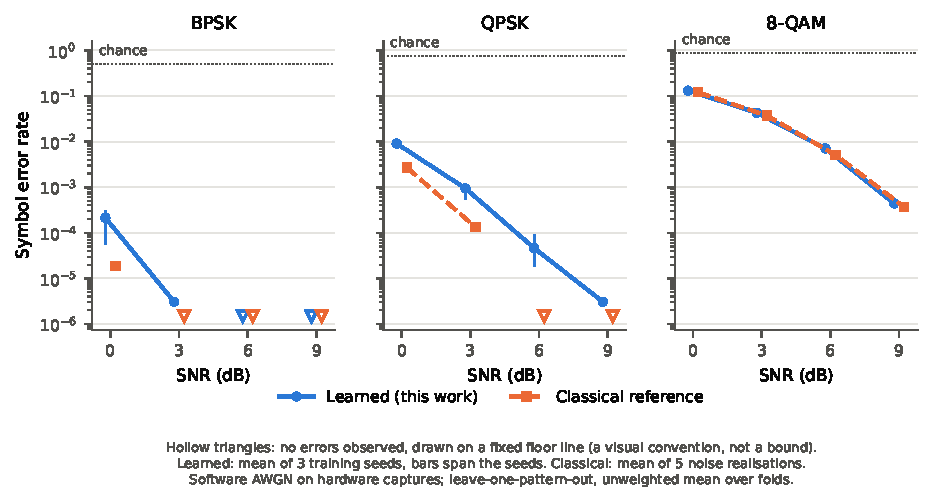
\includegraphics[width=\textwidth]{fig1_ser_vs_snr.pdf}
\caption{Symbol error rate against SNR for the learned and classical reference
receivers on the same leave-one-pattern-out test records, as the unweighted
mean over folds. SNR is the per-sample ratio of \eqref{eq:noise};
$E_s/N_0 = \mathrm{SNR} + 10$~dB. Learned: mean of three training seeds, with
bars spanning the seeds. Classical: mean of five noise realisations. Hollow
triangles mark operating points at which no error was observed in any run.
They are drawn on a fixed floor line at $1.5\times10^{-6}$, a plotting
convention below every non-zero mean, not a confidence bound.}
\label{fig:ser}
\end{figure*}

\begin{table}[!t]
\caption{Symbol error rate, learned (L) and classical reference (C) receivers,
on the same leave-one-pattern-out test records, as the unweighted mean over
folds. L is the mean of three training seeds; C is the mean of five noise
realisations. A dash means no error was observed in any run;
$<\!10^{-4}$ marks rates that are non-zero but below the last digit shown.}
\label{tab:ser}
\centering
\setlength{\tabcolsep}{4pt}
\begin{tabular}{lcccccc}
\toprule
& \multicolumn{2}{c}{BPSK} & \multicolumn{2}{c}{QPSK}
& \multicolumn{2}{c}{8-QAM} \\
\cmidrule(lr){2-3}\cmidrule(lr){4-5}\cmidrule(lr){6-7}
SNR & L & C & L & C & L & C \\
\midrule
$0$~dB & 0.0002 & $<\!10^{-4}$ & 0.0091 & 0.0027 & 0.1310 & 0.1206 \\
$3$~dB & $<\!10^{-4}$ & -- & 0.0009 & 0.0001 & 0.0429 & 0.0372 \\
$6$~dB & -- & -- & $<\!10^{-4}$ & -- & 0.0071 & 0.0051 \\
$9$~dB & -- & -- & $<\!10^{-4}$ & -- & 0.0004 & 0.0004 \\
$12$~dB & -- & -- & -- & -- & $<\!10^{-4}$ & 0.0002 \\
\bottomrule
\end{tabular}
\end{table}

At the lowest signal-to-noise ratios the reference receiver has the lower error
rate for all three modulations. At $0$~dB, 8-QAM gives $0.1310 \pm 0.0008$ (mean
$\pm$ standard deviation over seeds) against $0.1206 \pm 0.0016$, which is
$8.6\%$ higher. QPSK gives $0.0091 \pm 0.0012$ against $0.0027$, a factor of
$3.4$. Most of the QPSK difference comes from the Q1 fold, which trains on two
records: $0.0175$ against $0.0043$ and $0.0054$ for Q2 and Q3. BPSK makes $6$,
$19$ and $30$ errors in $57{,}472$ symbols across the three seeds, against about
one for the reference receiver. From $6$~dB, BPSK and QPSK differ by at most
ten errors in tens of thousands of symbols. For 8-QAM the gap narrows with
SNR: $0.0071$ against $0.0051$ at $6$~dB, and $0.00044$ against $0.00037$ at
$9$~dB.
At $12$~dB the learned receiver makes $5$--$18$ 8-QAM errors in $53{,}940$
symbols, depending on the seed, and none from $15$~dB. The reference receiver
keeps a floor of nine errors per realisation at every SNR from $12$~dB up.
Where Table~\ref{tab:ser} shows a dash, no error was observed. That bounds the
rate only loosely: errors within a record are not independent, so the usual
$3/N$ bound ($5\times10^{-5}$ for BPSK) is indicative only.

These results support comparable performance in the tested regime. They do not
establish equivalence, which we have not tested against any margin. A
reference receiver given the constellation and whole-record synchronisation is
close to the best a symbol-by-symbol detector can do on this channel, and we
interpret neither difference as a performance claim.

\begin{figure}[!t]
\centering
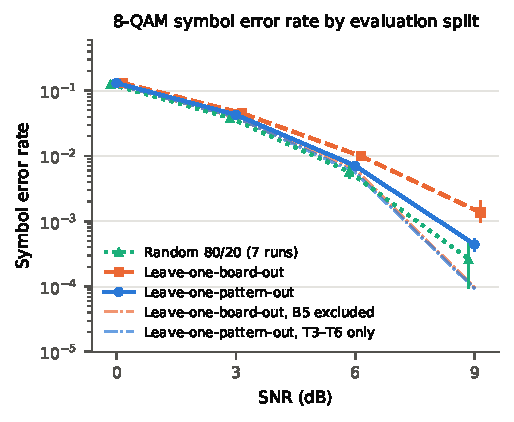
\includegraphics[width=\columnwidth]{fig2_no_memorisation.pdf}
\caption{8-QAM symbol error rate by evaluation split, as the unweighted mean
over folds. Bars span three training seeds; for the random split they span
seven runs (three seeds on the main partition and four further partitions).
The dash-dot lines are leave-one-board-out without board B5 and
leave-one-pattern-out without the T1+T2 fold, which trains on four records.}
\label{fig:splits}
\end{figure}

\subsection{Generalisation}
\label{sec:generalisation}

\begin{table*}[!t]
\caption{8-QAM symbol error rate by evaluation split, as the unweighted mean
over folds, mean $\pm$ standard deviation over runs. \emph{Runs}: training
seeds, or for the random split seeds and partitions. Leave-one-attenuation-out
has one seed. T3--T6 are the leave-one-pattern-out folds that train on
fourteen records.}
\label{tab:splits}
\centering
\setlength{\tabcolsep}{3pt}
\begin{tabular}{lcccc}
\toprule
Split (folds, runs) & $0$~dB & $3$~dB & $6$~dB & $9$~dB \\
\midrule
Random $80/20$ (1, 7) & 0.1256$\pm$0.0022 & 0.0383$\pm$0.0028 & 0.0057$\pm$0.0010 & 0.0003$\pm$0.0001 \\
Leave-one-pattern-out (5, 3) & 0.1310$\pm$0.0008 & 0.0429$\pm$0.0007 & 0.0071$\pm$0.0005 & 0.0004$\pm$0.0001 \\
\quad T3--T6 only (4, 3) & 0.1245$\pm$0.0024 & 0.0390$\pm$0.0007 & 0.0056$\pm$0.0006 & 0.0001$\pm$0.0002 \\
Leave-one-board-out (5, 3) & 0.1321$\pm$0.0007 & 0.0453$\pm$0.0017 & 0.0099$\pm$0.0007 & 0.0014$\pm$0.0006 \\
\quad without B5 (4, 3) & 0.1241$\pm$0.0008 & 0.0388$\pm$0.0014 & 0.0063$\pm$0.0007 & 0.0001$\pm$0.0001 \\
Leave-one-atten.-out (2, 1) & 0.1367 & 0.0452 & 0.0071 & 0.0004 \\
\bottomrule
\end{tabular}
\end{table*}

\emph{Withheld words.} Averaged over all five folds, holding out a word costs
$0.0054$ at $0$~dB: $0.1310$ against $0.1256$ for the random split. That is
larger than the spread across random-split runs ($0.0022$). The whole
difference comes from one fold. T1+T2 trains on only the four B1 records of
T3--T6 and tests on all five boards, so it combines a withheld word with four
unseen boards; it gives $0.1570 \pm 0.0058$. The four folds that withhold T3,
T4, T5 or T6 train on fourteen records across all five boards. They give
$0.1245 \pm 0.0024$, no worse than the random split at any SNR
(Table~\ref{tab:splits}). This is the comparison that Section~\ref{sec:bound}
sets up. On the random split, the test records carry training words, so the
neighbouring-symbol cues of Table~\ref{tab:context} and
Section~\ref{sec:controls} are available, and for T1 they determine the label.
On a withheld word they are not available. A receiver that exploited those
cues would do better on the random split. It does not, within the run-to-run
spread.

\emph{Withheld devices.} Leave-one-board-out is worse than
leave-one-pattern-out at $6$ and $9$~dB, but not uniformly across boards. Board
B5 gives $0.0246$ at $6$~dB and $0.0064$ at $9$~dB (mean of three seeds),
against $0.0057$--$0.0068$ and at most $0.0002$ for B1--B4. Without B5, the
leave-one-board-out mean is $0.1241$, $0.0063$ and $0.0001$ at $0$, $6$ and $9$~dB, no worse than leave-one-pattern-out. One
board in five does not transfer well. The rest transfer as well as a withheld
word.

Per-fold results are given in Table~\ref{tab:perfold}. Two folds are thin and
are reported with their training size: BPSK with the pseudorandom sequence held
out trains on a single record and QPSK with its primary word held out trains on
two. Both have the highest error rates in their modulation. Four of the five
8-QAM folds train on fourteen records. In those four folds, and in every BPSK
and QPSK fold except Q1 and PRBS63, the test set is a single record from
board B1 (Section~\ref{sec:dataset}-D). They show generalisation to a new word
on B1, not to a new word on unseen hardware.

% Seven columns do not fit one column of a two-column layout (73pt over).
% Promoted to a full-width float rather than shrinking the type further.
\begin{table*}[!t]
\caption{Per-fold results, training seed~0. \emph{Train records} is the number
of records in the training partition; the two folds with fewer than three are
the thin folds discussed in the text. \emph{Test symbols} counts evaluated
windows, after the edge trimming of Section~\ref{sec:conditioning}. The S1,
Q2, Q3 and T3--T6 folds each test a single record from board B1.
\emph{Position-only} is a lookup from a symbol's index within the data word to
its most frequent training label, against chance levels of $0.500$, $0.750$
and $0.875$. It is a meaningful control only where the withheld word is absent
from training. Every leave-one-board-out fold reuses the training word, so
position then determines the label exactly, and the entry is marked
\textit{n/a} (Section~\ref{sec:controls}).
}

\label{tab:perfold}
\centering
\begin{tabular}{llrrrrr}
\toprule
Modulation & Held out & Train records & Test symbols
& SER at $0$~dB & SER at $6$~dB & Position-only \\
\midrule
\textit{Leave-one-pattern-out} & & & & & & \\
BPSK & PRBS63 & 1 & 53{,}880 & 0.0001 & 0.0000 & 0.5290 \\
BPSK & S1 & 15 & 3{,}592 & 0.0000 & 0.0000 & 0.5003 \\
QPSK & Q1 & 2 & 35{,}950 & 0.0174 & 0.0001 & 0.7751 \\
QPSK & Q2 & 11 & 3{,}595 & 0.0042 & 0.0000 & 0.7502 \\
QPSK & Q3 & 11 & 3{,}595 & 0.0064 & 0.0000 & 0.8334 \\
8-QAM & T1+T2 & 4 & 39{,}556 & 0.1519 & 0.0119 & 0.8864 \\
8-QAM & T3 & 14 & 3{,}596 & 0.1310 & 0.0072 & 0.8749 \\
8-QAM & T4 & 14 & 3{,}596 & 0.1313 & 0.0028 & 0.7500 \\
8-QAM & T5 & 14 & 3{,}596 & 0.1271 & 0.0044 & 0.8751 \\
8-QAM & T6 & 14 & 3{,}596 & 0.1185 & 0.0064 & 0.8751 \\
\addlinespace
\textit{Leave-one-board-out} & & & & & & \\
BPSK & B1 & 12 & 14{,}368 & 0.0001 & 0.0000 & n/a \\
BPSK & B2 & 13 & 10{,}776 & 0.0000 & 0.0000 & n/a \\
BPSK & B3 & 13 & 10{,}776 & 0.0002 & 0.0000 & n/a \\
BPSK & B4 & 13 & 10{,}776 & 0.0000 & 0.0000 & n/a \\
BPSK & B5 & 13 & 10{,}776 & 0.0002 & 0.0000 & n/a \\
QPSK & B1 & 8 & 14{,}380 & 0.0070 & 0.0000 & n/a \\
QPSK & B2 & 10 & 7{,}190 & 0.0054 & 0.0000 & n/a \\
QPSK & B3 & 10 & 7{,}190 & 0.0049 & 0.0000 & n/a \\
QPSK & B4 & 10 & 7{,}190 & 0.0036 & 0.0000 & n/a \\
QPSK & B5 & 10 & 7{,}190 & 0.0174 & 0.0001 & n/a \\
8-QAM & B1 & 8 & 25{,}172 & 0.1287 & 0.0057 & n/a \\
8-QAM & B2 & 13 & 7{,}192 & 0.1194 & 0.0049 & n/a \\
8-QAM & B3 & 13 & 7{,}192 & 0.1193 & 0.0057 & n/a \\
8-QAM & B4 & 13 & 7{,}192 & 0.1283 & 0.0060 & n/a \\
8-QAM & B5 & 13 & 7{,}192 & 0.1675 & 0.0302 & n/a \\
\bottomrule
\end{tabular}
\end{table*}

\subsection{Negative controls}
\label{sec:controls}
\begin{table}[!t]
\caption{Controls on the leave-one-pattern-out folds, as the unweighted mean
over folds. \emph{Shuffled}: training labels permuted, test labels as
measured; mean over five permutation seeds, with the range of the five
fold-means in brackets. \emph{Position-only}: the lookup of the text, with
its cyclic-shift null mean in brackets. \emph{Context-only}: a lookup from the
true labels of the window's neighbouring symbols to the target label. Model:
learned receiver at $6$~dB, mean of three seeds. Chance is $1-1/K$.}
\label{tab:controls}
\centering
\footnotesize
\setlength{\tabcolsep}{1.8pt}
\begin{tabular}{lccccc}
\toprule
Mod. & Chance & Shuffled & Position & Context & Model \\
\midrule
BPSK & 0.500 & 0.549 [0.376, 0.750] & 0.5147 (0.4999) & 0.4959 & 0 \\
QPSK & 0.750 & 0.710 [0.579, 0.846] & 0.7862 (0.7477) & 0.6943 & $<\!10^{-4}$ \\
8-QAM & 0.875 & 0.922 [0.875, 0.977] & 0.8523 (0.8719) & 0.9001 & 0.0071 \\
\bottomrule
\end{tabular}
\end{table}

\emph{Shuffled labels.} The original control permuted labels across the
training \emph{and} test symbols of one leave-one-board-out fold. With the test
labels randomised, a chance-level score was guaranteed whatever the network
had learned, so the control could not fail. It has been replaced. Training
labels are now permuted within the training records of each
leave-one-pattern-out fold, the test labels are left as measured, and each fold
is run with five permutation seeds. Averaged over folds and seeds, the shuffled-label error rates are $0.549$, $0.710$ and $0.922$, against chance levels of $0.500$, $0.750$ and $0.875$ (Table~\ref{tab:controls}). Single runs scatter much more widely: from $0.169$ to $1.000$ for BPSK, $0.371$ to $0.917$ for QPSK and $0.625$ to $1.000$ for 8-QAM.
This is a property of the data rather than of the network. Each word offers only $8$ to $63$ distinct noise-free windows. A network trained on permuted labels learns an arbitrary but systematic function of the waveform, often close to a constant class. Its error rate on a test word then depends on which classes that word contains: on an 8-QAM word with six of the eight points, a constant prediction scores $0.75$ or $1.0$. A BPSK run can even converge on an inverted demodulator. On this corpus, a single shuffled run is therefore not a reliable chance reference, and runs below chance arise by the same mechanism.
What the control does establish is that no shuffled run comes near the trained receiver. On noise-free test windows the lowest shuffled-run error rate is $0.169$. The receiver's is zero on every leave-one-pattern-out fold, and at most $0.0071$ at $6$~dB. A path from input to target that bypassed the waveform, such as an index, an ordering or a leaked label, would let a network trained on permuted labels still score well on the true test labels. None does.

\emph{Context-only.} A third control measures the neighbouring context
that the bound leaves in the window. A lookup from the true labels of a
window's neighbours to its target label, fitted on the training records, gives
$0.4959$, $0.6943$ and $0.9001$ on the withheld words (Table~\ref{tab:controls}), against chance levels of $0.500$, $0.750$ and $0.875$. The cues of Table~\ref{tab:context} do not transfer between words. On splits that reuse the training word they do: QPSK context then gives $0.583$--$0.596$. For 8-QAM the window holds no neighbour. If the previous symbol could be read through the interference of Section~\ref{sec:bound}, however, a lookup from it would give $0.625$ on the random split and $0.132$ on leave-one-board-out (zero on four of the five boards), against $0.902$ on leave-one-pattern-out. Section~\ref{sec:generalisation} finds no corresponding advantage for the receiver on those splits.

\emph{Trace readability.} The context-only control uses true labels. It does
not ask whether the network can read a neighbour through the trace of
Section~\ref{sec:bound}, so we asked the network directly. The 8-QAM network
was trained as in Section~\ref{sec:arch} to name the label of the previous, or
the next, symbol from its target-only window. The test favours the shortcut.
There is one network per record, trained on the first $75\%$ of the record and
tested on the last $25\%$, so the word, the board and the positions are those
it trained on. It is scored only where the target's class cannot give the
answer away: at the four positions in each of T3--T6 whose point occurs twice
with different neighbours. There, a predictor that knows the target's class
exactly is right $0.501$ of the time. Over four words, both neighbours and
three seeds, the network is right $0.500$ and $0.501$ of the time on
noise-free windows, and less often at low SNR, where it also misreads the
target. Trained on noise-free windows only, it reaches $0.507$ and $0.497$.
With the neighbour inside the window, the same procedure names it correctly
$0.89$--$0.93$ of the time at $0$~dB and in every run at least $0.999$ of the
time from $15$~dB, so the probe works. The trace is measurable in the waveform averaged over hundreds of word
repetitions; the network does not read it from a single window.

Physics explains why reading it would not help. At the SNRs where the receiver
makes 8-QAM errors, $0$ to $12$~dB (Table~\ref{tab:ser}), the energy of the
trace is $2$ to $18$~dB below the noise in the symbol interval: $E_s/N_0$ is
the SNR plus $10$~dB, and the trace lies $24$--$28$~dB below $E_s$. It reaches
the noise level only near $15$~dB, from which the receiver makes no 8-QAM
errors left to correct.

\emph{Position-only.} The position-only control requires a qualification that is easy to overlook. Labels are
a periodic tiling of the transmitted word, so a symbol's index within that word
determines its label exactly. Across all $148$ pairs of records carrying the same
word---including pairs drawn from different boards and different
attenuations---the label sequences are identical up to a cyclic shift. A
predictor reading only the symbol index therefore attains a symbol error rate of
zero on any split whose test partition reuses a training word, which is the case
for every leave-one-board-out, leave-one-attenuation-out and random fold. On
those splits the position-only figure is not a control and we do not report it.

It is a control on leave-one-pattern-out, where the withheld word is absent from
training and is not a cyclic shift of any training word: the best cyclic
agreement between distinct words is $0.500$ for QPSK and $0.375$ for 8-QAM,
against chance agreements of $0.250$ and $0.125$. There the lookup gives
$0.5147$, $0.7862$ and $0.8523$ (Table~\ref{tab:controls},
Fig.~\ref{fig:controls}). The nominal chance levels $1-1/K$ are not the right
reference for single folds, because a word has few symbols and an unequal
class mix. We therefore form a null for each fold. The lookup's predicted word
is applied at every one of its cyclic shifts, which keeps its class mix and
destroys any alignment with the test word. The null means are $0.4999$,
$0.7477$ and $0.8719$. A lookup that had learned something transferable would
place the true alignment at or near the best of its shifts. In nine of the ten
folds, other shifts do better: for QPSK, $10$, $7$ and $8$ of the $11$ other
shifts give a lower error rate than the observed $0.7751$, $0.7502$ and
$0.8334$. For T4, the observed alignment is the best of the eight. An
unaligned lookup lands there with probability $1/8$, which is unremarkable in
one fold of ten. The position-only lookup therefore does no better than an
unaligned copy of itself, which is the sense in which it is at chance.

This concerns the control, not the receiver. The network is given a window of
waveform samples and nothing else: it receives no symbol index and classifies
each window independently, so on no split can it exploit the positional
redundancy that defeats the lookup.

\begin{figure}[!t]
\centering
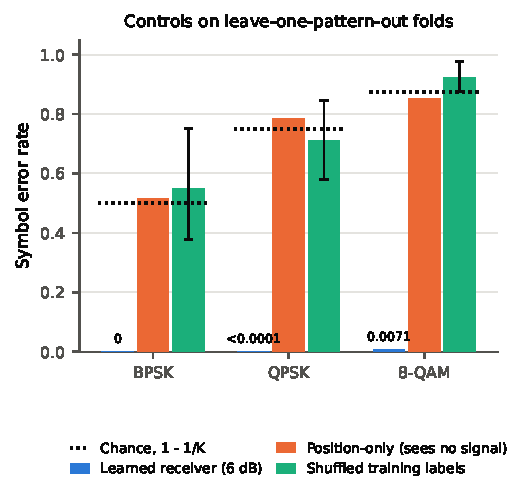
\includegraphics[width=\columnwidth]{fig3_controls.pdf}
\caption{Controls on the leave-one-pattern-out folds. Learned receiver at $6$~dB, mean of three seeds. Position-only lookup. Shuffled training labels, mean of five permutation seeds, with bars spanning the five fold-means. Dotted lines mark the nominal chance level $1-1/K$; the spread of the shuffled control is discussed in the text.}
\label{fig:controls}
\end{figure}

\subsection{Positive control: a longer window}
\label{sec:positive}
The comparisons above find no sign that the bounded receiver exploits the
transmitted sequence. That finding would mean little if the evaluation could
not detect such exploitation when it occurs. We therefore removed the bound and
repeated the evaluation.

\begin{table}[!t]
\caption{Positive control: the network of Section~\ref{sec:arch} with the
bound removed. Symbol error rate at $0$~dB, with noise-free test windows in
brackets; 0 means no errors. \emph{Context}: neighbouring symbols before and
after the target. \emph{Blanked}: the long window with the target and its two
nearest neighbours set to zero before noise is added. \emph{Seen}: test records
of three random $80/20$ partitions whose exact word occurs in training, mean
over partitions. \emph{Withheld}: leave-one-pattern-out, unweighted mean over
folds. Training seed~0. All three inputs are scored on the same symbols.}
\label{tab:positive}
\centering
\footnotesize
\setlength{\tabcolsep}{3pt}
\begin{tabular}{llccc}
\toprule
Mod. & Input & Context & Seen & Withheld \\
\midrule
8-QAM & Bounded & 0     & 0.1231 (0) & 0.1301 (0) \\
      & Long    & 4+4   & 0.0010 (0) & 0.6221 (0.5756) \\
      & Blanked & 4+4   & 0.0052 (0) & 0.8809 (0.8976) \\
\addlinespace
QPSK  & Bounded & 1+0   & 0.0055 (0) & 0.0096 (0) \\
      & Long    & 6+6   & 0 (0)      & 0.3115 (0.2995) \\
      & Blanked & 6+6   & 0.0003 (0) & 0.7524 (0.7365) \\
\addlinespace
BPSK  & Bounded & 2+2   & 0 (0)      & $<\!10^{-4}$ (0) \\
      & Long    & 10+10 & $<\!10^{-4}$ (0) & 0.0463 (0.0381) \\
      & Blanked & 10+10 & 0.0004 (0) & 0.5058 (0.5078) \\
\bottomrule
\end{tabular}
\end{table}

\emph{Design.} The long input holds four neighbouring symbols on each side of
the target for 8-QAM, six for QPSK and ten for BPSK. By enumeration on the
measured labels, three on each side for 8-QAM and QPSK, and five for BPSK,
already determine every label of every word, even with the target and its two
nearest neighbours removed. The \emph{blanked} input is the long window with
exactly those three symbols set to zero before noise is added. The blanked span
exceeds the $\pm 0.88$-symbol support of the anti-alias filter, so no filtered
copy of the target remains in the window. Whatever the blanked network labels
correctly, it labels from the sequence. Loss, optimiser, epochs and training
SNR range are those of Section~\ref{sec:arch}. Only the strides change, to fit
the longer input, which raises the parameter count to $24{,}202$, $29{,}190$
and $39{,}364$ for 8-QAM, QPSK and BPSK. Each record loses the same edge
symbols under all three inputs, so they are scored on identical symbols.

\emph{Leakage.} Every record repeats one short word, so the test needs care.
Splits are by record, as throughout. No withheld word is a cyclic shift of a
training word under any constellation rotation; the one such pair, T1 and T2,
is already a single group. A lookup from the true labels of the long context,
fitted on the training records, stays at or near chance on every
leave-one-pattern-out fold: $0.504$, $0.750$ and $0.850$ for BPSK, QPSK and
8-QAM, and $0.825$ for 8-QAM if every training word is also entered under each
rotation. The withheld words therefore offer no context that a training word
supplies. On the random partitions, each test record is classed by whether its
exact word occurs in training. A T2 record counts as unseen when only T1 is
trained. In the one partition where that arises, the long-window network did
not carry the sequence of T1 over to its rotated copy.

\emph{Result.} On seen words, the long-window network makes almost no errors at
$0$~dB (Table~\ref{tab:positive}). For 8-QAM it gives $0.0010$, against
$0.1231$ for the bounded window on the same symbols and about $0.12$ for the
classical reference receiver (Table~\ref{tab:ser}). No receiver that decides
each symbol from its own waveform can do this. The network is predicting
symbols from the word. The blanked network shows this directly. It never sees
the target, yet on seen words it labels it with an error rate of $0.0052$ at
$0$~dB and without error on noise-free windows.

On withheld words the same networks fail. The blanked network falls to chance.
The long-window network, which does see the target, does far worse than the
bounded one, and noise is not the cause: on noise-free windows it mislabels
$0.5756$ of the 8-QAM and $0.2995$ of the QPSK symbols, where the bounded
network mislabels none. Given the context, the network learns the training
words in preference to the symbol, and a new word misleads it. For BPSK the
effect sits in one fold. With S1 withheld the network trains on fifteen PRBS63
records and reads the symbol ($0.0003$ at $0$~dB). With PRBS63 withheld it
trains on the single S1 record and mislabels $0.0761$ of the noise-free PRBS63
windows.

\emph{What it shows.} Three things follow. First, the network can memorise,
and it does so as soon as its input allows. Noise was added throughout
training, so noise does not prevent memorisation. It makes the context more
useful, not less. Second, a random split rewards memorisation, here by two
orders of magnitude at $0$~dB, and on this corpus it cannot tell memorisation
from demodulation. Third, leave-one-pattern-out exposes it. Under the bounded
window neither signature appears. Seen and withheld words give $0.1231$ and
$0.1301$ for 8-QAM, and $0.0055$ and $0.0096$ for QPSK. The QPSK difference
comes from the Q1 fold, which trains on two records; without it the withheld
mean is $0.0056$. The same holds at $-6$~dB, below the training range, where a
partial context cue would help most. Without the two thin folds, T1+T2 and Q1,
seen and withheld words give $0.408$ and $0.407$ for 8-QAM, and $0.142$ and
$0.143$ for QPSK. The control was run with one training seed. Its effects
exceed the seed spread of Section~\ref{sec:generalisation} by more than two
orders of magnitude.

\subsection{Constellation geometry}
\label{sec:geometry}
\begin{figure*}[!t]
\centering
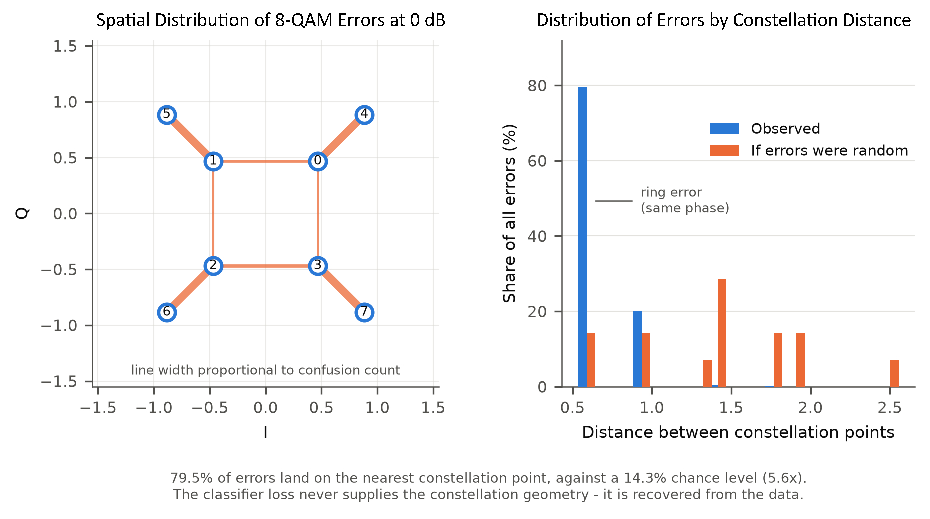
\includegraphics[width=\textwidth]{fig5_error_geometry.pdf}
\caption{Destination of 8-QAM errors at $0$~dB. The figure comes from a separate
training run with board B2 withheld (leave-one-board-out, $18$ epochs,
$\lambda = 0.2$, seed~0), with one noise realisation: $863$ errors among
$7{,}192$ test symbols. Left: confusions drawn on the unit-RMS reference
constellation, with line width proportional to count. Each line combines both
directions of a confusion; the two directions differ by $9.6\%$ of all errors
in total. Pairs with fewer than five confusions are not drawn. Right: share of
errors against inter-point distance, compared with a null in which every wrong
class is equally likely.}
\label{fig:geometry}
\end{figure*}

The constellation term of \eqref{eq:loss} was ablated at
$\lambda \in \{0,\,0.2,\,1.0\}$ in a separate, smaller run: one
leave-one-board-out fold (B2 withheld), 18 epochs and one seed
(Table~\ref{tab:ablation}). Its absolute values therefore differ from
Table~\ref{tab:splits}; the main run gives $0.1194$ and $0.0049$ on the same
fold at $0$ and $6$~dB. The three values of $\lambda$ differ by at most
$0.0030$ at $0$~dB, less than the seed spread of
Section~\ref{sec:generalisation}. \emph{The constellation term does not improve
error rate.}

\begin{table}[!t]
\caption{Ablation of the constellation term of \eqref{eq:loss}. One
leave-one-board-out fold (B2 withheld), 18 epochs, one seed; the main results
use $\lambda = 0.2$ and 25 epochs.}
\label{tab:ablation}
\centering
\begin{tabular}{lcccc}
\toprule
& \multicolumn{3}{c}{8-QAM} & QPSK \\
\cmidrule(lr){2-4}\cmidrule(lr){5-5}
$\lambda$ & $0$~dB & $3$~dB & $6$~dB & $0$~dB \\
\midrule
$0.0$ & 0.1246 & 0.0370 & 0.0060 & 0.0058 \\
$0.2$ & 0.1261 & 0.0359 & 0.0056 & 0.0051 \\
$1.0$ & 0.1276 & 0.0364 & 0.0058 & 0.0054 \\
\bottomrule
\end{tabular}
\end{table}

Nor does it make the latent head reproduce the constellation. Retrained at
$\lambda = 0.2$, the head returns the same output for every input: all eight
8-QAM class means lie within $0.02$ of one point, all four QPSK class means lie
at one point, and the spread within each class is at most $0.005$. That
constant satisfies the penalty while carrying no information about the symbol,
the degenerate solution noted in Section~\ref{sec:arch}. A penalty tied to each
symbol's \emph{true} class would avoid the collapse, but would supply the
geometry as supervision. We therefore do not present the head as evidence of
recovered geometry.

The classifier's errors, by contrast, follow the geometry. In the run of
Fig.~\ref{fig:geometry}, $79.5\%$ of the $863$ 8-QAM errors at $0$~dB land on
the nearest constellation point, against $14.3\%$ if every wrong class were
equally likely; for QPSK, all $33$ do, against $66.7\%$. This is the pattern
additive noise produces in any receiver that discriminates by waveform
distance. It is not a test of memorisation, since a model that had memorised
waveform prototypes would err the same way. That question is addressed in
Sections~\ref{sec:controls} and~\ref{sec:positive}.

\subsection{The boards' own demodulators}
\label{sec:hardware}
As a side result, the captures characterise the boards' own BPSK demodulators,
measured against the known transmitted sequence on the fifteen PRBS63 records
(Fig.~\ref{fig:lock}). Agreement is the best agreement of the TP-9 output with
PRBS63 over all 63 cyclic shifts and both polarities. On random sequences the
same maximisation gives $66.6\%$, with 95th percentile $69.8\%$
(Section~\ref{sec:groundtruth}-C). All eleven records at or below $509$~mV
output level are consistent with chance; two exceed the 95th percentile
marginally, at $71.4\%$ and $73.0\%$, about what eleven draws from the null
produce. All four records at or above $626$~mV agree at $92$--$100\%$. No
record falls between the two levels, so the threshold lies in that interval but
is not fixed by these data. One board's BPSK path delivers only $391$~mV and
never locks, although its QPSK and 8-QAM outputs match the other boards'. The
boards' QPSK demodulator failed to lock on the primary QPSK word on every unit,
so no hardware QPSK baseline exists.

Self-consistency is not a valid lock criterion. On one board at $329$~mV,
self-consistency read $0.979$ while agreement with the transmitted sequence was
at chance: the unlocked demodulator had settled into a stable period-two state,
inverting its output every word period. Four records in this study would have
been wrongly classed as locked by that metric. Lock should be established only
against a known transmitted sequence.

\begin{figure}[!t]
\centering
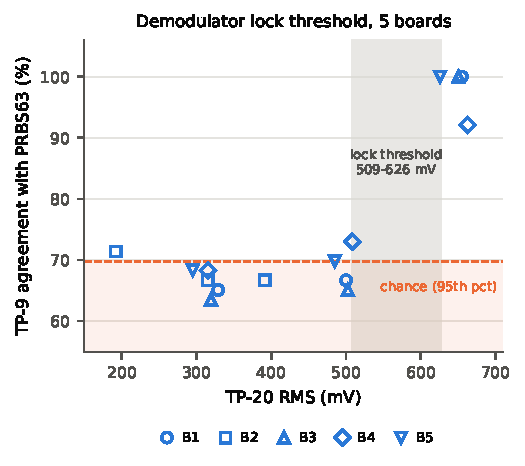
\includegraphics[width=\columnwidth]{fig4_lock_threshold.pdf}
\caption{Behaviour of the boards' own BPSK demodulators on the PRBS63 word,
across five boards: agreement of TP-9 with the transmitted sequence against
TP-20 output level. The shaded band is the chance region up to the 95th
percentile of the null ($69.8\%$), from the best agreement over 63 cyclic
shifts and both polarities. Records at or below $509$~mV are consistent with
chance; records at or above $626$~mV agree at $92$--$100\%$. No record falls
between the two levels.}
\label{fig:lock}
\end{figure}

% =====================================================================
\section{Discussion}

The principal result of this work is methodological. When a learned receiver is
trained on a periodic transmitted sequence, held-out evaluation alone does not
establish that the receiver demodulates. Part of the property can instead be
imposed. If the input window is cut shorter than the context complexity of
every transmitted word, no window determines its label by lookup, whatever the
model's capacity or training procedure. That guarantee is narrow. It does not
remove partial predictability of the context, and it does not remove the
inter-symbol interference that carries a weak trace of neighbouring symbols
into the window.

The empirical tests address what the bound leaves open. On splits that reuse a
training word the neighbouring context is far more informative than on
leave-one-pattern-out; for 8-QAM T1, one preceding symbol determines the label.
A receiver that exploited the context through interference would therefore
score better on the random split than on leave-one-pattern-out. Against the
withheld-word folds with comparable training data it does not, beyond the
spread across seeds and partitions. The one fold that is worse, T1+T2, trains
on four records from a single board (Section~\ref{sec:generalisation}).
The corrected shuffled-label control adds a second, weaker check
(Section~\ref{sec:controls}). The positive control of
Section~\ref{sec:positive} shows that these tests can detect what they look
for. Lengthened past the bound, the same network memorises the words: the
random split rewards it by two orders of magnitude, and the withheld words
expose it. Under the bound, neither signature appears. None of this is a
proof. Together with the bound, it makes sequence exploitation an unlikely
explanation of the error rates reported here.

We note that the bound is cheap to adopt. It requires the context complexity of
the transmitted words, computable by enumeration from the measured labels, and
an input window cut accordingly. Where a test sequence has high complexity the
constraint is loose. Where the words are short, as in much laboratory practice,
it is tight. Without it, a random split can overstate a receiver by two orders
of magnitude (Section~\ref{sec:positive}).

The comparison of Section~\ref{sec:ser} should be read in this light. The
classical reference receiver is given resources the network is not: the
constellation's decision regions, a carrier search band, carrier and phase
estimates from the whole record, and resolution of the phase ambiguity against
the labels. It is also built from the same operations as the label procedure.
It has the lower error rate at the lowest signal-to-noise ratios. The learned
receiver comes close to it without being given the carrier frequency, the
constellation geometry or the decision boundaries. It is not equivalent to it,
and we make no equivalence claim.

The cross-device gap is narrower than it first appears. Leave-one-board-out is
worse than leave-one-pattern-out at $6$ and $9$~dB because of one board, B5.
Without B5, the leave-one-board-out mean is no worse than leave-one-pattern-out
(Section~\ref{sec:generalisation}). One board in five transfers poorly. That
makes device-invariant training worth pursuing, but five boards cannot show
how common such a board is.

% =====================================================================
\section{Limitations}
\label{sec:limitations}

\emph{Content diversity.} The corpus is large in noise realisations and hardware
variation but small in distinct transmitted content: 8-QAM comprises five
independent 24-bit words, or 40 distinct symbol instances.

\emph{Device count and design.} Five functional units support a five-fold
cross-device evaluation. The device-to-device differences we observe are large
enough to be measured, but the sample is too small to characterise their
distribution. The design is not crossed: the additional words S1, Q2, Q3 and
T2--T6 exist only on board B1, so those leave-one-pattern-out folds test new
words on one board, and pattern and device effects cannot be separated for
them. Recording every word on every board is the remedy.

\emph{Scope of the bound.} The bound excludes deterministic lookup of a label
from the neighbouring symbols in its window. It does not exclude partial
predictability (Table~\ref{tab:context}) or the neighbouring-symbol trace left
by the transmitter's pulse response, measured at $-18.5$ to $-27.9$~dB
(Section~\ref{sec:bound}). That these are not exploited is an empirical finding
of Sections~\ref{sec:generalisation}, \ref{sec:controls}
and~\ref{sec:positive}, not a consequence of the bound.

\emph{Offline, record-level processing.} The labels, the symbol timing and the
AGC are each computed from the complete record. The AGC uses the record's
noise-free RMS (Section~\ref{sec:conditioning}). The network does not see the
label path, but its windows inherit the record-level timing and gain. The
receiver is therefore a classifier of pre-synchronised, pre-normalised
windows, not a streaming receiver.

\emph{Run-to-run variation.} Three training seeds were run on the folds the
comparisons rest on, and a single seed elsewhere. With so few seeds and
partitions, differences smaller than the seed spread reported in
Section~\ref{sec:generalisation} cannot be resolved. The positive control of
Section~\ref{sec:positive} used one seed; its effects are far larger than that
spread.

\emph{Synthetic noise.} The hardware supplies the carrier, the filter
response, quantisation and device-to-device variation, while additive white
Gaussian noise is applied in software. The boards' own noise control contributes
approximately $+0.02$~dB within the signal band and is unusable as a
signal-to-noise axis.

\emph{Symbol timing is supplied.} The receiver is given neither the carrier
frequency nor any description of the pulse shape. Its input window is
symbol-synchronous, however, which supplies the symbol rate and the sampling
phase, and the waveform it sees is shaped by the physical transmit pulse. This is not incidental: under a
one-symbol window for 8-QAM, timing cannot be recovered from the window
itself, so the context bound and timing-blindness cannot both hold. The system
should be described as operating on symbol-synchronous windows from a
conventional timing front-end~\cite{gardner1986ted}.

\emph{Carrier sensitivity does not support a robustness claim.} A classical
receiver's dependence on carrier knowledge is often cited as a disadvantage. We
did not find it to be one. A blind carrier estimate from eight symbols
($13.3$~ms) is off by $1.02$~Hz, but over those eight symbols that offset
rotates the phase by only $4.9^{\circ}$, and they demodulate without error.
Estimate error and tolerance shrink together, and the classical receiver was
self-consistent at every observation length tested, from 8 to $3{,}596$
symbols. We therefore claim no robustness advantage for the learned receiver.

\emph{8-QAM labels are classes, not bits.} The tribit carried by each 8-QAM
constellation point is not resolved (Section~\ref{sec:groundtruth}-C). The
8-QAM results concern constellation-point classification.

\emph{Operating regime.} A single carrier frequency, a single symbol rate, and
an additive Gaussian channel without multipath or fading. Generalisation beyond
this regime is not evidenced here.

% =====================================================================
\section{Conclusion}
We have presented a hardware dataset of 43 dual-channel captures from five
distinct communication trainer boards, together with a convolutional receiver
whose input window always holds fewer neighbouring symbols than are needed to
determine its label, for every transmitted word in the corpus. The bound
excludes deterministic lookup from the window's context by construction. The
remaining routes, partial predictability and inter-symbol interference, are
measured and tested rather than assumed away. A positive control shows that
the bound is needed: given a longer window, the same network labels symbols
from the transmitted word instead of the waveform, which a random split rewards
and held-out words expose. The receiver comes close to a
classical reference receiver on BPSK, QPSK and star 8-QAM without being given
the carrier frequency, the constellation or the decision boundaries. It
operates on symbol-synchronous windows with record-level gain control, under
software-added Gaussian noise. Its errors concentrate on the nearest
constellation neighbours. Two negative results are reported. A
constellation-geometry loss term does not improve error rate, and its latent
output collapses to a single point. A classical receiver's dependence on
carrier knowledge did not, under measurement, constitute a practical
disadvantage.

Future work should address the limitations that bound the present study
most tightly: the number of distinct transmitted words, the restriction of the
additional words to a single board, and the number of devices. These set the
resolution of the leave-one-pattern-out and cross-device evaluations.

% =====================================================================
\section*{Acknowledgment}
% \todonote{acknowledgment}{%
This research was carried out in the Communication Laboratory of the Department of Information and Communication Technology (ICT), Bangladesh University of Professionals (BUP). The authors express sincere gratitude to the department for providing access to the laboratory facilities. Special thanks are extended to Mr. Syed Abul Qayyum, Laboratory Technician  for his technical support and assistance throughout the experimental phase of this work.

\todonote{AI-use disclosure}{IEEE requires AI-generated content (text, figures,
code) to be disclosed here, naming the system, the sections affected and the
level of assistance; language editing alone is outside the policy but
disclosure is recommended. This revision was drafted with Claude (Anthropic),
including substantive text in Sections I, II, IV--VIII. State the actual
use of ChatGPT, Claude and Gemini accurately before submission.}

\todonote{prior dissemination}{Disclose the accepted WorldCUR 2027 abstract in
the submission letter (and cite it here if it is archived), and state how this
article extends it.}

\bibliographystyle{IEEEtran}
\bibliography{refs}

% =====================================================================
% \todonote{author biographies}{%
% IEEE Access requires a short biography and a photograph for each author, placed
% here after the references. Use the \texttt{IEEEbiography} environment from the
% class documentation; the photograph is passed as the optional argument as a
% $1\,\text{in}\times1.25\,\text{in}$ \texttt{includegraphics} with
% \texttt{keepaspectratio}.}

\begin{IEEEbiography}[{
\includegraphics[width=1in,height=1.25in,clip,keepaspectratio]{khalid.jpeg}}]{Mohammad Khalid Hasan Nabil}
is currently pursuing the B.Sc. degree in Information and Communication Engineering with Bangladesh University of Professionals (BUP), Dhaka, Bangladesh. 

% He conducts research in the university's Communication Laboratory focusing on hardware-implemented neural receivers and deep learning for digital signal processing. His broader research interests include scientific and physics-informed machine learning, surrogate modeling, physical-layer communications, and deep learning for digital demodulation.
\end{IEEEbiography}

\begin{IEEEbiography}[{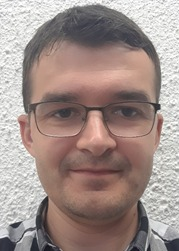
\includegraphics[width=1in,height=1.25in,clip,keepaspectratio]{ivan.jpeg}}]{Ivan Grgi\'{c}}
received the Ph.D. degree in mechanical engineering. He is currently an Assistant Professor with the Mechanical Engineering Faculty in Slavonski Brod, University of Slavonski Brod, Slavonski Brod, Croatia.
\end{IEEEbiography} 

\begin{IEEEbiography}[{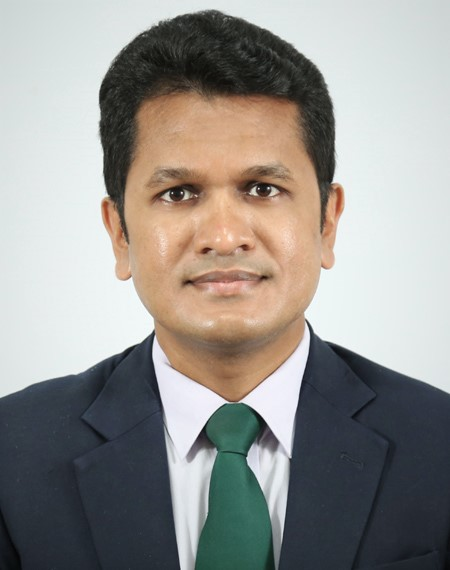
\includegraphics[width=1in,height=1.25in,clip,keepaspectratio]{mainul.jpeg}}]{Md. Maynul Islam}
is currently an Assistant Professor with the Department of Information and Communication Technology, Bangladesh University of Professionals, Dhaka 1216, Bangladesh.
\end{IEEEbiography}


% \EOD closes an IEEE Access manuscript.
\EOD

\end{document}
